% Options for packages loaded elsewhere
\PassOptionsToPackage{unicode}{hyperref}
\PassOptionsToPackage{hyphens}{url}
\PassOptionsToPackage{dvipsnames,svgnames,x11names}{xcolor}
%
\documentclass[
  letterpaper,
  number,
  review,
  3p]{elsarticle}

\usepackage{amsmath,amssymb}
\usepackage{iftex}
\ifPDFTeX
  \usepackage[T1]{fontenc}
  \usepackage[utf8]{inputenc}
  \usepackage{textcomp} % provide euro and other symbols
\else % if luatex or xetex
  \usepackage{unicode-math}
  \defaultfontfeatures{Scale=MatchLowercase}
  \defaultfontfeatures[\rmfamily]{Ligatures=TeX,Scale=1}
\fi
\usepackage{lmodern}
\ifPDFTeX\else  
    % xetex/luatex font selection
\fi
% Use upquote if available, for straight quotes in verbatim environments
\IfFileExists{upquote.sty}{\usepackage{upquote}}{}
\IfFileExists{microtype.sty}{% use microtype if available
  \usepackage[]{microtype}
  \UseMicrotypeSet[protrusion]{basicmath} % disable protrusion for tt fonts
}{}
\makeatletter
\@ifundefined{KOMAClassName}{% if non-KOMA class
  \IfFileExists{parskip.sty}{%
    \usepackage{parskip}
  }{% else
    \setlength{\parindent}{0pt}
    \setlength{\parskip}{6pt plus 2pt minus 1pt}}
}{% if KOMA class
  \KOMAoptions{parskip=half}}
\makeatother
\usepackage{xcolor}
\setlength{\emergencystretch}{3em} % prevent overfull lines
\setcounter{secnumdepth}{5}
% Make \paragraph and \subparagraph free-standing
\ifx\paragraph\undefined\else
  \let\oldparagraph\paragraph
  \renewcommand{\paragraph}[1]{\oldparagraph{#1}\mbox{}}
\fi
\ifx\subparagraph\undefined\else
  \let\oldsubparagraph\subparagraph
  \renewcommand{\subparagraph}[1]{\oldsubparagraph{#1}\mbox{}}
\fi


\providecommand{\tightlist}{%
  \setlength{\itemsep}{0pt}\setlength{\parskip}{0pt}}\usepackage{longtable,booktabs,array}
\usepackage{calc} % for calculating minipage widths
% Correct order of tables after \paragraph or \subparagraph
\usepackage{etoolbox}
\makeatletter
\patchcmd\longtable{\par}{\if@noskipsec\mbox{}\fi\par}{}{}
\makeatother
% Allow footnotes in longtable head/foot
\IfFileExists{footnotehyper.sty}{\usepackage{footnotehyper}}{\usepackage{footnote}}
\makesavenoteenv{longtable}
\usepackage{graphicx}
\makeatletter
\def\maxwidth{\ifdim\Gin@nat@width>\linewidth\linewidth\else\Gin@nat@width\fi}
\def\maxheight{\ifdim\Gin@nat@height>\textheight\textheight\else\Gin@nat@height\fi}
\makeatother
% Scale images if necessary, so that they will not overflow the page
% margins by default, and it is still possible to overwrite the defaults
% using explicit options in \includegraphics[width, height, ...]{}
\setkeys{Gin}{width=\maxwidth,height=\maxheight,keepaspectratio}
% Set default figure placement to htbp
\makeatletter
\def\fps@figure{htbp}
\makeatother
% definitions for citeproc citations
\NewDocumentCommand\citeproctext{}{}
\NewDocumentCommand\citeproc{mm}{%
  \begingroup\def\citeproctext{#2}\cite{#1}\endgroup}
\makeatletter
 % allow citations to break across lines
 \let\@cite@ofmt\@firstofone
 % avoid brackets around text for \cite:
 \def\@biblabel#1{}
 \def\@cite#1#2{{#1\if@tempswa , #2\fi}}
\makeatother
\newlength{\cslhangindent}
\setlength{\cslhangindent}{1.5em}
\newlength{\csllabelwidth}
\setlength{\csllabelwidth}{3em}
\newenvironment{CSLReferences}[2] % #1 hanging-indent, #2 entry-spacing
 {\begin{list}{}{%
  \setlength{\itemindent}{0pt}
  \setlength{\leftmargin}{0pt}
  \setlength{\parsep}{0pt}
  % turn on hanging indent if param 1 is 1
  \ifodd #1
   \setlength{\leftmargin}{\cslhangindent}
   \setlength{\itemindent}{-1\cslhangindent}
  \fi
  % set entry spacing
  \setlength{\itemsep}{#2\baselineskip}}}
 {\end{list}}
\usepackage{calc}
\newcommand{\CSLBlock}[1]{\hfill\break\parbox[t]{\linewidth}{\strut\ignorespaces#1\strut}}
\newcommand{\CSLLeftMargin}[1]{\parbox[t]{\csllabelwidth}{\strut#1\strut}}
\newcommand{\CSLRightInline}[1]{\parbox[t]{\linewidth - \csllabelwidth}{\strut#1\strut}}
\newcommand{\CSLIndent}[1]{\hspace{\cslhangindent}#1}

\usepackage{rotating}
\makeatletter
\@ifpackageloaded{bookmark}{}{\usepackage{bookmark}}
\makeatother
\makeatletter
\@ifpackageloaded{caption}{}{\usepackage{caption}}
\AtBeginDocument{%
\ifdefined\contentsname
  \renewcommand*\contentsname{Table of contents}
\else
  \newcommand\contentsname{Table of contents}
\fi
\ifdefined\listfigurename
  \renewcommand*\listfigurename{List of Figures}
\else
  \newcommand\listfigurename{List of Figures}
\fi
\ifdefined\listtablename
  \renewcommand*\listtablename{List of Tables}
\else
  \newcommand\listtablename{List of Tables}
\fi
\ifdefined\figurename
  \renewcommand*\figurename{Figure}
\else
  \newcommand\figurename{Figure}
\fi
\ifdefined\tablename
  \renewcommand*\tablename{Table}
\else
  \newcommand\tablename{Table}
\fi
}
\@ifpackageloaded{float}{}{\usepackage{float}}
\floatstyle{ruled}
\@ifundefined{c@chapter}{\newfloat{codelisting}{h}{lop}}{\newfloat{codelisting}{h}{lop}[chapter]}
\floatname{codelisting}{Listing}
\newcommand*\listoflistings{\listof{codelisting}{List of Listings}}
\makeatother
\makeatletter
\makeatother
\makeatletter
\@ifpackageloaded{caption}{}{\usepackage{caption}}
\@ifpackageloaded{subcaption}{}{\usepackage{subcaption}}
\makeatother
\journal{WSTLUR Symposium 2024}
\ifLuaTeX
  \usepackage{selnolig}  % disable illegal ligatures
\fi
\usepackage{bookmark}

\IfFileExists{xurl.sty}{\usepackage{xurl}}{} % add URL line breaks if available
\urlstyle{same} % disable monospaced font for URLs
\hypersetup{
  pdftitle={Where's dinner coming from? A utility-based investigation of access to nutrition in Utah.},
  pdfauthor={Gregory S. Macfarlane; Emma Stucki; Myrranda Salmon; Alisha H. Redelfs; Lori A. Spruance},
  pdfkeywords={Accessibility, Access to nutrition, Passive location
data},
  colorlinks=true,
  linkcolor={blue},
  filecolor={Maroon},
  citecolor={Blue},
  urlcolor={Blue},
  pdfcreator={LaTeX via pandoc}}

\setlength{\parindent}{6pt}
\begin{document}

\begin{frontmatter}
\title{Where's dinner coming from? A utility-based investigation of
access to nutrition in Utah.}
\author[1]{Gregory S. Macfarlane%
\corref{cor1}%
}
 \ead{gregmacfarlane@byu.edu} 
\author[1]{Emma Stucki%
%
}

\author[1]{Myrranda Salmon%
%
}

\author[2]{Alisha H. Redelfs%
%
}

\author[2]{Lori A. Spruance%
%
}


\affiliation[1]{organization={Civil and Construction Engineering
Department, Brigham Young University},city={Provo, Utah
USA},postcode={84602},postcodesep={}}
\affiliation[2]{organization={Public Health Department, Brigham Young
University},city={Provo, Utah USA},postcode={84602},postcodesep={}}

\cortext[cor1]{Corresponding author}





        
\begin{abstract}
Convenient access to high-quality nutrition is a critical element of
public health as well as an important interface between communities and
the transportation system. In this research, we seek to construct a
detailed picture of the nutrition environment in three communities in
Utah, alongside the community members' ability to access that
environment through multiple transportation modes. In doing so we
construct a utility-based accessiblity model enabled by modern mobility
device data. This model reveals the tradeoffs between the quality and
price of goods on one hand and the distance traveled to reach them on
the other. We then apply this model to a series of potential
access-improving policies: building a new store, improving an existing
store, and improving the non-automobile transport network between
residents and existing stores. The results show that new or improved
store locations bring substantially higher benefits than improvements to
the transportation system, at likely lower costs. The findings suggest
that transportation agencies work to increase the availability of
community-sized grocery stores in low-access areas, and consider
activity-based methods of measuring resource access.
\end{abstract}





\begin{keyword}
    Accessibility \sep Access to nutrition \sep 
    Passive location data
\end{keyword}
\end{frontmatter}
    
\bookmarksetup{startatroot}

\section{Introduction}\label{introduction}

The ability of people to access quality nutrition has been studied at
length in public health and urban geography for decades (Beaulac et al.,
2009; Walker et al., 2010). This interest is motivated in large part by
an observed spatial disparity in nutrition access in many communities
--- though this issue may be particularly pronounced in the United
States (Beaulac et al., 2009). The spatial disparity has been linked at
an aggregate level with negative public health outcomes (Chen et al.,
2016; Cooksey-Stowers et al., 2017), though other complicating factors
including prices and habits may be present as well (Ghosh-Dastidar et
al., 2014).

At the same time, access to nutrition and to community resources in
general is frustratingly hard to define. ``Accessibility'' is an
abstract concept without a specific quantitative definition (Handy \&
Niemeier, 1997). However, using accessibility as a policy measure
requires comparative quantification, and transportation and public
health researchers have constructed several quantitative measures, such
as presence of a store within a travel time buffer, or the distance to
the nearest store. These measures are relatively easy to calculate using
readily available GIS software, but elide much useful information (Dong
et al., 2006; Logan et al., 2019). These types of measures require the
researcher to make a series of assumptions and assertions: why is 30
minutes chosen instead of 40? Is that time by transit or highway or
walking? Should these definitions change for individuals in different
socioeconomic groups? And people do not always go to the closest grocery
store to begin with (Clifton, 2004; Hillier et al., 2011); how much
further are people willing to travel to go to a store that is cheaper or
that has a wider variety of goods? And perhaps the home location isn't
the only spatial point of reference (Liu et al., 2022). A measure that
potentially combines many of these different considerations is
desirable.

In this research, we develop and explore an accessibility measure based
on destination choice models estimated for three distinct communities in
Utah. This methodology is based on a unique dataset made by linking
between three extensive data sources:

\begin{enumerate}
\def\labelenumi{\arabic{enumi}.}
\tightlist
\item
  A detailed survey of the nutrition market in three Utah communities.
\item
  Location-based services data derived from mobile phone records
  revealing which grocery stores are frequented by residents of
  different neighborhoods.
\item
  Multi-modal network data providing detailed mobility data by car,
  walking, and public transit.
\end{enumerate}

These data will be combined in order to develop accurate logit models
that demonstrate the variables that are significant to grocery store
choice in Utah. These models could then be used to find accessibility to
stores and impact transportation policy to improve quality of life for
all communities in Utah.

This paper is organized in a typical manner. A methodology for data
collection and modeling is described in Section~\ref{sec-methods} and a
description of the nutrition environment and choice models estimates
follows in Section~\ref{sec-results}. Section~\ref{sec-scenarios}
presents a series of scenarios to which we apply the models estimated in
Section~\ref{sec-results}, illustrating the interrelated elements of
nutrition quality and transportation infrastructure in developing more
complete access to nutrition.

\bookmarksetup{startatroot}

\section{Methods}\label{sec-methods}

This section describes how we construct a model of access to grocery
stores in communities in Utah. We first describe the theoretical model,
and then describe data collection efforts to estimate this model and
apply it.

\subsection{Model}\label{model}

A typical model of destination choice (Recker \& Kostyniuk, 1978) can be
described as a random utility maximization model where the utility of an
individual \(i\) choosing a particular destination \(j\) is
\begin{equation}\phantomsection\label{eq-utility}{ U_{ij} = \beta_{s}f(k_{ij}) + \beta_{x}(X_j) }\end{equation}
where \(f(k_{ij})\) is a function of the travel impedance or costs from
\(i\) to \(j\) and \(X_{j}\) represents the location attributes of
\(j\). The coefficients \(\beta\) can be estimated given sufficient data
revealing the choices of individuals. The probability that individual at
location \(i\) will choose alternative \(j\) from a choice set \(J\) can
be estimated with a multinomial logit model (MNL) (McFadden, 1974),
\begin{equation}\phantomsection\label{eq-mnl}{ P_i(j) = \frac{\exp(U_{ij})}{\sum_{j' \in J}{\exp(U_{ij'})}}}\end{equation}
The overall fit of the model can be described with the Akaike
Information Criterion (AIC) --- which should be minimized --- or by the
McFadden likelihood ratio
\(\rho^2_0 = 1 - \ln\mathcal{L} / \ln\mathcal{L}_0\). In this ratio
\(\ln{\mathcal{L}}\) is the model log-likelihood and
\(\ln{\mathcal{L}_0}\) the log-likelihood of an alternative model where
all destinations are equally likely; a higher \(\rho^2_0\) value
indicates more explanatory power relative to this null, random chance
only model.

The idea of using destination choice logsums as accessibility terms is
not new, and the theory for doing so is described in (Ben-Akiva \&
Lerman, 1985, p. 301). Effectively, the natural logarithm of the
denominator in Equation~\ref{eq-mnl} represents the consumer surplus ---
or total benefit --- available to person \(i\):

\begin{equation}\phantomsection\label{eq-cs}{ CS_i = \ln\left(\sum_{j \in J} \exp(U_{ij})\right)}\end{equation}

A difference in logsum measures may exist for a number of reasons that
affect the utility functions described in Equation~\ref{eq-utility}. For
example, individuals at different locations or with different mobility
will see different impedance values \(k_{ij}\) and therefore affected
utility. Changes to the attributes of the destinations \(X_j\) will
likewise affect the utility.

Despite the relative maturity of this theory, applications of
utility-based access in the literature are still rare, outside of public
transport forecasting analyses (Geurs et al., 2010). The rarity is
likely explained by an unfamiliarity with destination choice models and
the ready availability of simpler methods on one hand (Logan et al.,
2019), and the difficulty in obtaining a suitable estimation dataset for
particular land uses on the other (Kaczynski et al., 2016). This second
limitation has been somewhat improved by a new methodology developed by
(Macfarlane et al., 2022), relying on commercial location-based services
data to estimate the affinity for simulated agents to visit destinations
of varying attributes and distances.

\subsection{Data}\label{data}

In this research, we develop a unique dataset to estimate the
destination choice utility coefficients for grocery store choice in
three different communities in Utah. The three communities were selected
to maximize potential observed differences in utility between community
residents. The three communities are Utah County, West Salt Lake County,
and San Juan County. Note that in this document we refer to the second
community as ``Salt Lake'' even though this does not refer to the entire
Salt Lake County nor to Salt Lake City, rather, we focus on communities
in the western part of the valley, such as Magna, Kearns, and West
Valley City.

Table~\ref{tbl-acsdata} shows several key population statistics based on
2021 American Community Survey data for block groups in the three
communities of interest. Utah County is a largely suburban county with
high incomes and a low percentage of minority individuals. The Salt Lake
region is more dense with somewhat lower incomes and household sizes but
a high share of minority individuals. San Juan County is primarily
rural, with a few small communities and a large reservation for the
Navajo Tribe.

\begin{table}

\caption{\label{tbl-acsdata}Demographic Statistics of Study Region}

\centering{

\centering
\begin{tabular}[t]{lrrr}
\toprule
 & Utah & Salt Lake & San Juan\\
\midrule
Total population & 627,098 & 655,830 & 7,091\\
Total households & 171,538 & 216,731 & 2,090\\
Housing units per sq. km & 599 & 831 & 103\\
Median income & 79,453 & 64,868 & 58,586\\
Percent minority individuals & 18 & 36 & 26\\
\bottomrule
\end{tabular}

}

\end{table}%

Estimating the utility model described in Equation~\ref{eq-mnl} for
grocery stores requires three interrelated data elements:

\begin{enumerate}
\def\labelenumi{\arabic{enumi}.}
\tightlist
\item
  An inventory of grocery store attributes \(X_j\);
\item
  A representative travel impedance matrix \(K\) composed of all
  combinations of origin \(i\) and destination \(j\);
\item
  A database of observed person flows between \(i\) and \(j\) by which
  to estimate the \(\beta\) coefficients. We describe each of these
  elements in turn in the following sections.
\end{enumerate}

\subsubsection{Store Attributes}\label{store-attributes}

The store attributes were collected using the Nutritional Environment
Measures Survey --- Stores (NEMS-S) tool (Glanz et al., 2007). This tool
was developed to reveal significant differences in the availability and
cost of healthy foods in an environment, and has been validated for this
purpose. Beyond superficial attributes such as the store category
(dollar store, convenience store, ethnic market, etc.) and the number of
registers, the NEMS-S collects detailed information about numerous store
offerings such as the availability of produce, dairy products, lean
meats, juices, and canned and dry goods of various specific types. Of
particular interest to the survey are availability and price
differentials of lower-fat alternatives: for example, the survey
instrument requests the shelf space allocated to milk products of
various fat levels and the price of each product.

Student research assistants collected the store attributes by visiting
grocery stores, dollar stores, ethnic markets, and other food markets in
the three communities of interest described above. Stores were
identified using internet-based maps combined with in-person validation
and observation. The student researchers completed the NEMS-S instrument
with the aid of a digital survey and a tablet computer. Each researcher
who collected data was trained to use the survey at a control store in
Provo, and the training data helped to eliminate the risk of surveyor
bias. The store attributes were collected in the spring of 2021 for Utah
County and spring of 2022 for Salt Lake and San Juan Counties. In Utah
and Salt Lake Counties, we included dollar stores and grocery stores but
did not include convenience stores. Given the rural nature of San Juan
County, we made two adjustments to capture the entirety of the nutrition
environment. First, we included convenience stores and trading posts if
they were the only food market in a community. We also included
full-service grocery stores in Cortez, Colorado, and Farmington, New
Mexico in the San Juan data collection, as community conversations made
it clear that many residents will drive these long distances for
periodic shopping with greater availability and lower prices.

Using the information in the NEMS-S survey, two measures of a store can
be calculated: an availability score based on whether stores stock
particular items as well as lower-calorie options; and a cost score
describing the spread between prices of these options. These score
values are described in (Lunsford et al., 2021), and we developed an R
package to compute the scores; this package is available at
\url{https://github.com/byu-transpolab/nemsr}. In the availability
score, each store is given a value for whether or not there are more
healthful options available in the store, such as low-calorie chips, or
low-fat milk. If the store does not have a more healthful option in a
category it receives a lower score, so stores with more availability of
healthful food options will receive a higher availability score. For the
cost score, the measure is the price spread between healthful and less
healthful options: if the price of whole wheat bread is cheaper than
white bread, the store receives positive points for the cost option, if
the price is the same then zero points are awarded, and if the wheat
bread is more expensive then the store receives negative points. Thus a
store with a higher availability and cost score will have both more
healthful options, and a more advantageous pricing scheme towards those
options.

One important store attribute that the NEMS-S instrument does not
collect or compute directly is a measure of the cost of common goods
that can be compared across stores. We therefore used the data collected
from the NEMS-S instrument to construct a market basket-based
affordability measure that could be compared across stores, following
the approach of (Hedrick et al., 2022). This market basket score is
based on the US Department of Agriculture (USDA) 2021 Thrifty Food Plan
(FNS, 2021), which calculates a reference market basket for a family of
four. Because this market basket contains more (and sometimes different)
items than what the NEMS-S instrument requests, we chose relevant items
from our NEMS-S data as replacements. For example, the USDA market
basket contains a certain amount of poultry, but the NEMS-S score
collects the per-pound cost of ground beef at various fat contents. For
any stores that were missing any of the elements in the market basket,
we first substituted with another ingredient that would fit the
nutritional requirements. If no substitute was available, we included
the average price of the missing good at other stores in that community
multiplied by 1.5 as a penalty for not containing the product. The final
market basket score is the total cost of all foods in the market basket.
These costs can then be compared from store to store to understand
general affordability comparisons between stores.

\begin{table}

\caption{\label{tbl-nems}Grocery Store Attributes}

\centering{

\centering
\resizebox{\linewidth}{!}{
\begin{tabular}[t]{llrrrrrr}
\toprule
\multicolumn{2}{c}{ } & \multicolumn{2}{c}{Utah (N=63)} & \multicolumn{2}{c}{Salt Lake (N=39)} & \multicolumn{2}{c}{San Juan (N=50)} \\
\cmidrule(l{3pt}r{3pt}){3-4} \cmidrule(l{3pt}r{3pt}){5-6} \cmidrule(l{3pt}r{3pt}){7-8}
  &    & Mean & Std. Dev. & Mean & Std. Dev. & Mean & Std. Dev.\\
\midrule
Registers (incl. self checkout) &  & 12.5 & 11.7 & 9.9 & 8.9 & 6.1 & 8.8\\
NEMS-S availability score &  & 18.7 & 8.4 & 16.2 & 8.1 & 13.2 & 7.6\\
NEMS-S cost score &  & 1.9 & 2.3 & 2.3 & 2.2 & 1.9 & 1.9\\
Market basket cost &  & 126.1 & 21.5 & 141.6 & 19.2 & 157.6 & 16.8\\
\midrule
 &  & N & Pct. & N & Pct. & N & Pct.\\
Type & Convenience Store & 2 & 3.2 & 0 & 0.0 & 10 & 20.0\\
 & Dollar Store & 5 & 7.9 & 11 & 28.2 & 15 & 30.0\\
 & Grocery Store & 50 & 79.4 & 27 & 69.2 & 19 & 38.0\\
 & Other & 6 & 9.5 & 1 & 2.6 & 6 & 12.0\\
Pharmacy & FALSE & 42 & 66.7 & 32 & 82.1 & 43 & 86.0\\
 & TRUE & 21 & 33.3 & 7 & 17.9 & 7 & 14.0\\
Ethnic market & FALSE & 55 & 87.3 & 30 & 76.9 & 47 & 94.0\\
 & TRUE & 8 & 12.7 & 9 & 23.1 & 3 & 6.0\\
Other merchandise sold & FALSE & 52 & 82.5 & 35 & 89.7 & 47 & 94.0\\
 & TRUE & 11 & 17.5 & 4 & 10.3 & 3 & 6.0\\
\bottomrule
\end{tabular}}

}

\end{table}%

Table~\ref{tbl-nems} presents the store attribute data collected for
each community. Utah County generally has the largest average store size
(as measured by the number of checkout registers) while having the
lowest market basket cost, the highest availability of healthful food
(measured by the NEMS-S availability score) and the lowest difference
between healthy and unhealthy food (the NEMS-S cost score). San Juan
County has the smallest average stores, highest costs, and the lowest
availability of healthy options, and Salt Lake falls in between.

\subsubsection{Imputation of Missing Store
Data}\label{imputation-of-missing-store-data}

We collected detailed store attributes for stores in Utah County, San
Juan County, and a portion of Salt Lake County using the NEMS-S survey
instrument. These attributes form the basis of the choice models used to
determine access, but understanding access in other parts of Salt Lake
City or the state of Utah requires us to impute the attributes onto the
stores that we did not collect.

To do this, we used web-based mapping databases (including OpenStreetMap
and Google Maps) to obtain a list of grocery stores, dollar stores, and
appropriate convenience stores throughout the state. From this search,
we were able to determine each store's location, brand name, and store
type, which we also collected in the manual data assembly efforts. Using
this information, we built a multiple imputation model using the
\texttt{mice} package for R (van Buuren \& Groothuis-Oudshoorn, 2011).
The predictor variables in the imputation included the store brand and
type, as well as the average income and housing density in the nine
closest block groups to the store location (based on population-weighted
block group centroids and Euclidean distances).

\begin{figure}

\centering{

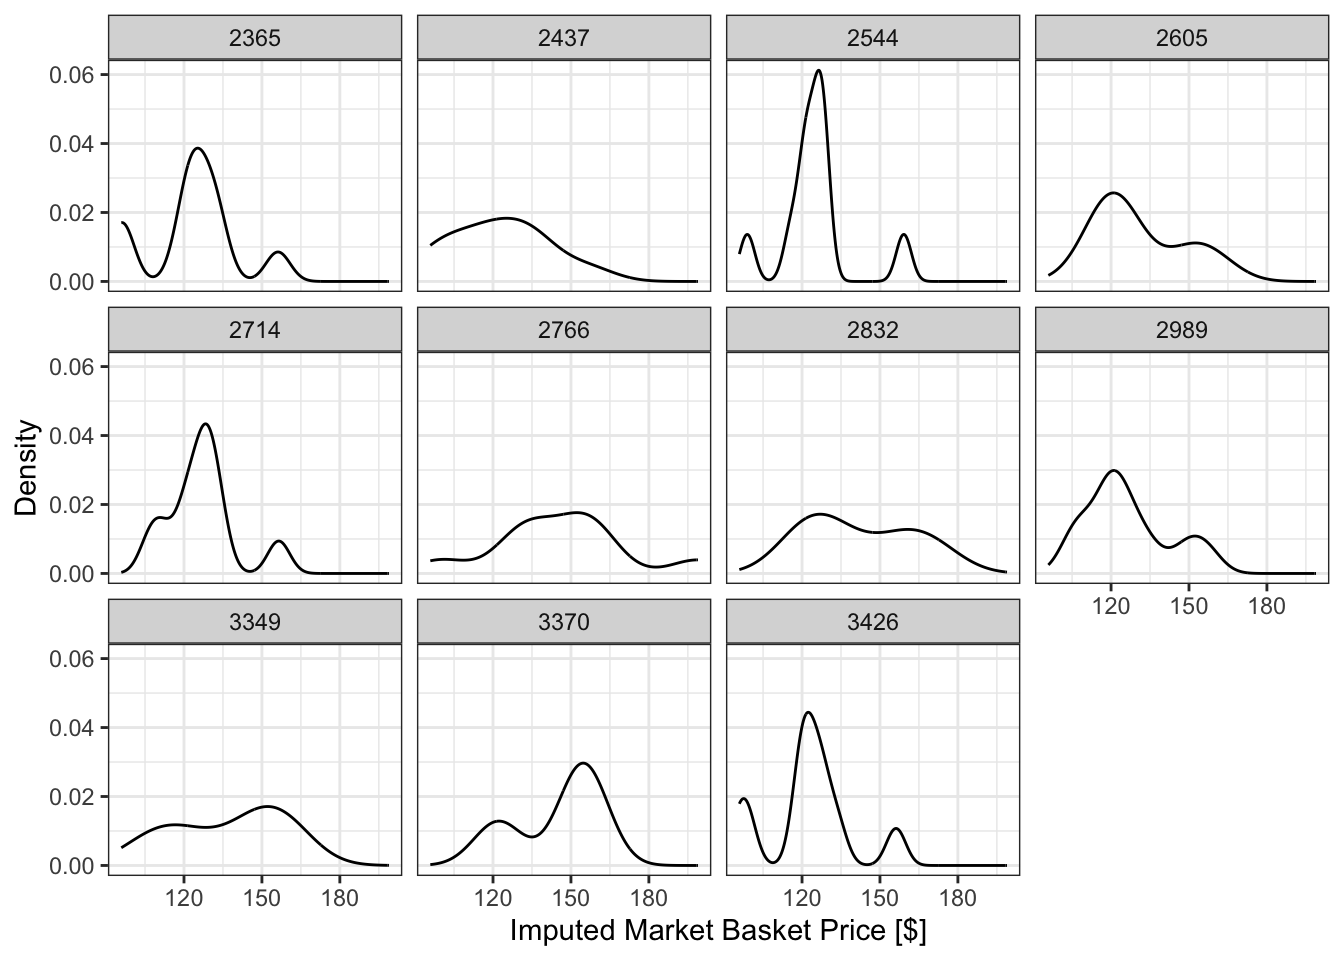
\includegraphics[width=5in,height=\textheight]{03_methods_files/figure-pdf/fig-marketimp-1.pdf}

}

\caption{\label{fig-marketimp}Imputed market price values for 15 random
grocery stores.}

\end{figure}%

Thirty iterations of the multiple imputation algorithm were run for each
of ten independent imputations. Figure~\ref{fig-marketimp} shows the
density of the ten imputed market basket prices for a randomly selected
set of 15 stores. As the figure reveals, there is some general peaking
in the predicted market price for most stores, but the imputation model
still predicts a wide range of possible prices for most stores. When
using the imputed data for analysis, we take the mean of the ten
predictions for continuous values, and the mode for discrete values.

\subsubsection{Travel Impedances}\label{sec-mcls}

The second element of the utility equation in Equation~\ref{eq-utility}
is the travel impedance between \(i\) and \(j\). Many possibilities for
representing this impedance exist, from basic euclidean distance to
complex network paths. A primary purpose of the model we are developing
in this research is to study comparative tradeoffs between
infrastructure-focused and environment-focused improvements to the
nutrition access of households. It is therefore essential that we use a
travel impedance measure that can combine and compare the cost of
traveling by multiple modes so that highway improvements and transit /
active transport improvements can be compared in the same basic model.

Just as the log-sum of a destination choice model is a measure that sums
the utility of multiple destination attributes and costs in a rigorous
manner, the log-sum of a mode choice model combines the utilities of all
available travel modes. In this study we assert the following mode
choice utility equations: \begin{align*} 
  V_{\mathrm{auto}, ij} &= -0.028(t_{\mathrm{auto}, ij})\\
  V_{\mathrm{bus}, ij} &= -4 -0.028(t_{\mathrm{bus}, ij}) -0.056(t_{\mathrm{wait}, ij}) -0.056(t_{\mathrm{access}, ij})\\
  V_{\mathrm{walk, ij}} &= -5 -0.028(t_{\mathrm{walk}, ij}) -1.116(d_{ij<1.5}) -5.58(d_{ij>1.5})\\
\end{align*} where \(t\) is the in-vehicle travel time in minutes for
each mode between \(i\) and \(j\). The transit utility function
additionally includes the wait time for transit as well as the time
necessary to access the transit mode on both ends by walking. The walk
utility includes a per-mile distance disutility that increases for
distances greater than 1.5 miles. These equations and coefficients are
adapted from a statewide mode choice model developed for UDOT research
(Barnes, 2021).

The log-sum, or total weighted impedance by all modes is therefore
\begin{equation}\phantomsection\label{eq-mcls}{
k_{ij} = \ln(e^{V_{\mathrm{auto}, ij}} + e^{V_{\mathrm{bus}, ij}} + e^{V_{\mathrm{walk},ij}})
}\end{equation}

In this implementation, \(i\) is the population-weighted centroid of a
2020 Census block group, and \(j\) is an individual grocery store. We
measure the travel times from each \(i\) to each \(j\) using the
\texttt{r5r} implementation of the R5 routing engine (Conway et al.,
2017, 2018; Conway \& Stewart, 2019; Pereira et al., 2021). This
algorithm uses common data elements --- OpenStreetMap roadway and active
transport networks alongside General Transit Feed Specification (GTFS)
transit service files --- to simulate multiple realistic route options
by all requested modes. We obtained OpenStreetMap networks and the Utah
Transit Authority GTFS file valid for May 2023 and requested the minimum
total travel time by each mode of auto, transit, and walking for a
departure between 8 AM and 9 AM on May 10, 2023. The total allowable
trip time by any mode was set to 120 minutes, and the walk distance was
capped at 10 kilometers; if a particular \(i,j\) pair exceeded these
parameters then the mode was presumed to not be available and
contributes no utility to the log-sum.

\subsubsection{Mobile Device Data}\label{mobile-device-data}

The final element of destination utility presented in
Equation~\ref{eq-utility} is the set of coefficients, which are often
estimated from household travel surveys in a travel demand context. It
is unlikely, however, that typical household diaries would include
enough trips to grocery stores and similar destinations to create a
representative sample.

Emerging mobile device data, however, could reveal the typical home
locations for people who are observed in the space of a particular
store. (Macfarlane et al., 2022) present a method for estimating
destination choice models from such data, which we repeat in this study.
We provided a set of geometric polygons for the grocery stores of
interest to StreetLight Data, Inc., a commercial location-based services
aggregator and reseller. StreetLight Data in turn provided data on the
number of mobile devices observed in each polygon grouped by the
inferred residence block group of those devices during summer 2022. We
then created a simulated destination choice estimation dataset for each
community resource by sampling 10,000 block group - grocery store
``trips'' from the StreetLight dataset. This created a ``chosen''
alternative; we then sampled ten additional stores from the same
community at random (each simulated trip was paired with a different
sampled store) to serve as the non-chosen alternatives. Random sampling
of alternatives is a common practice that results in unbiased estimates,
though the standard errors of the estimates might be larger than could
be obtained through a more carefully designed sampling scheme (Train,
2009).

\bookmarksetup{startatroot}

\section{Results}\label{sec-results}

This section presents results on the nutrition environment in each of
the three communities of Utah County, West Salt Lake County, and San
Juan County, along with destination choice model estimates and their
application to creating accessibility maps of each community and the
entire state of Utah.

\subsection{Nutrition Environment}\label{sec-nems}

Though some basic descriptive statistics of the grocery store attributes
were presented in Table~\ref{tbl-nems}, some additional exploration of
these attributes is valuable to understand the nutrition environment in
these three communities.

\begin{figure}

\centering{

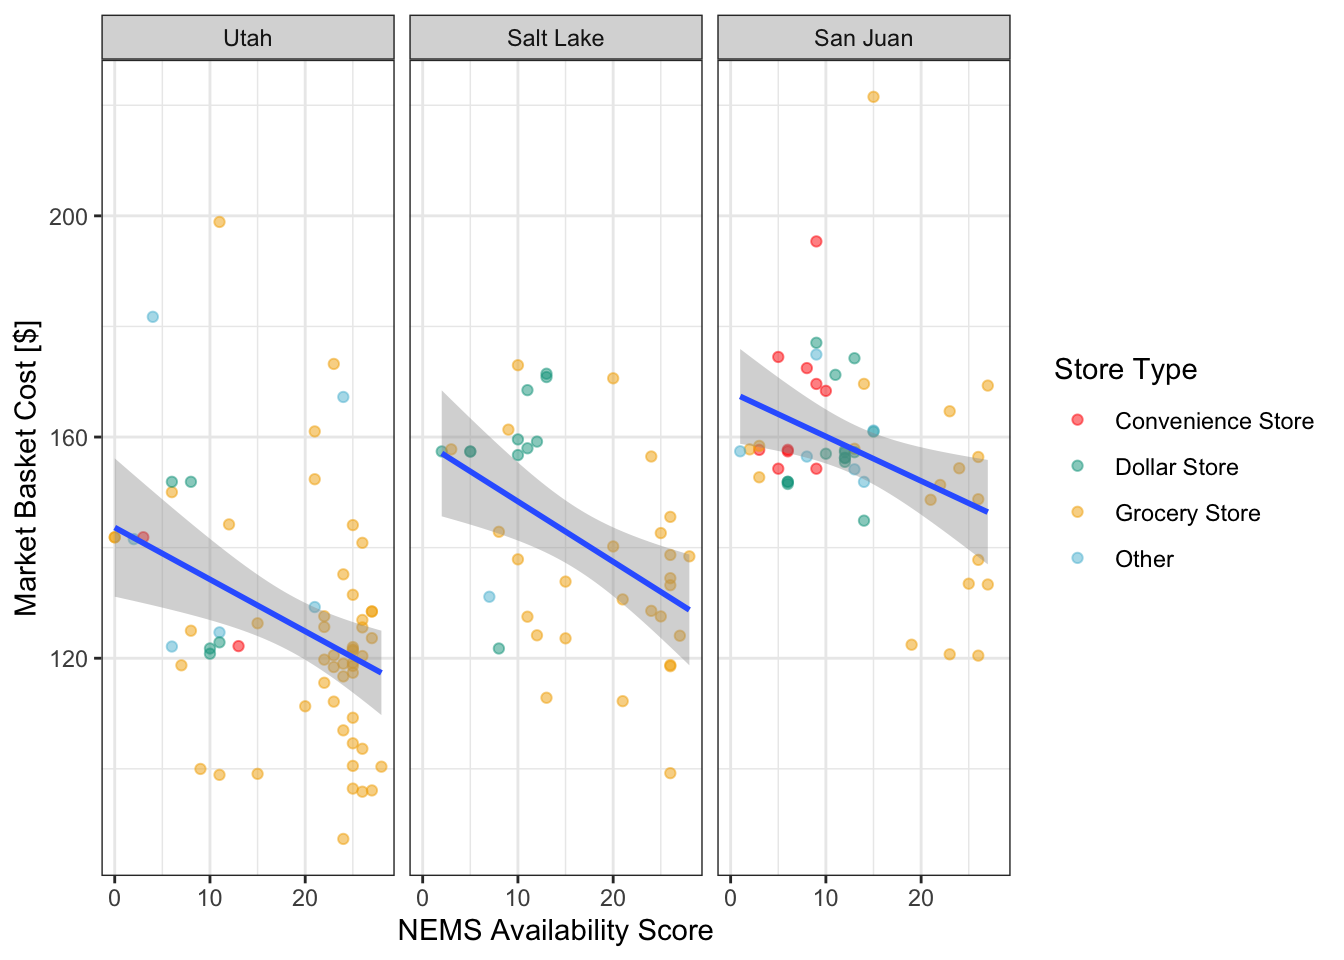
\includegraphics{04_estimation_files/figure-pdf/fig-nems-market-avail-1.pdf}

}

\caption{\label{fig-nems-market-avail}Relationship between NEMS
availability score and market basket score in each study community. Utah
county prices adjusted for 2021-2022 annual inflation.}

\end{figure}%

Figure~\ref{fig-nems-market-avail} presents the relationship between the
recorded NEMS availability score and the USDA market basket cost at the
stores by community and store type. In all three communities, the
relationship is strongly negative, with stores that stock more varieties
of goods also having overall lower prices for those goods. This is
emphasized by the bottom-right quadrants of these plots (high
availability, low-cost) being dominated by full-service grocery stores,
which have more availability and lower prices than convenience stores or
dollar stores, but require higher traffic and demand to make up for
their lower profit margins. Average prices in Utah County are lower than
prices in the other two communities across the availability spectrum;
this is true even after adjusting for 9.4\% annual inflation between
March 2021 and March 2022 in food products (Bureau of Labor Statistics,
2023).

\begin{figure}

\centering{

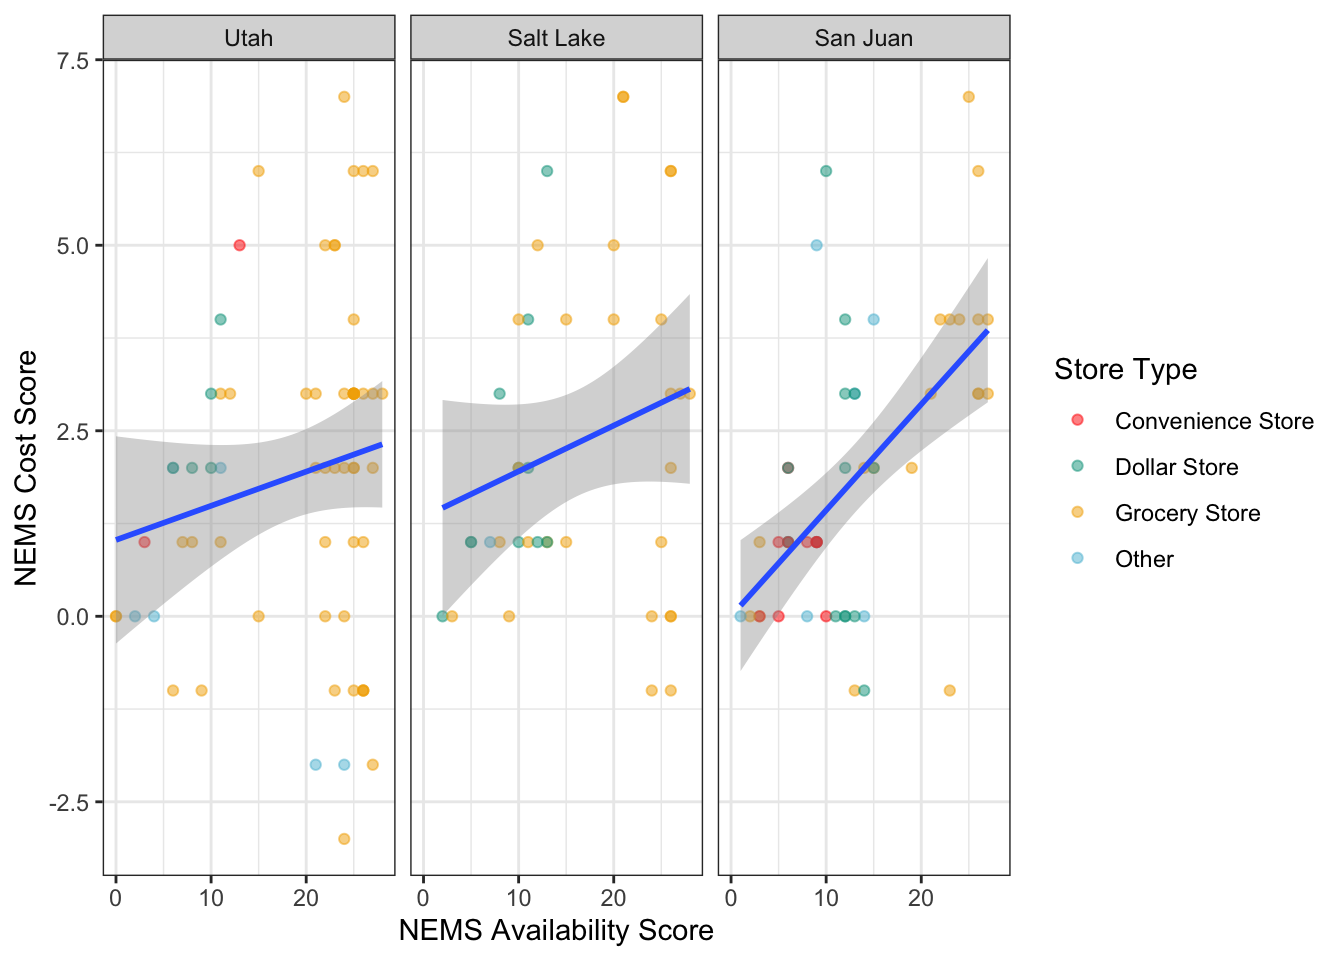
\includegraphics{04_estimation_files/figure-pdf/fig-nems-cost-avail-1.pdf}

}

\caption{\label{fig-nems-cost-avail}Relationship between NEMS
availability score and cost score in each study community.}

\end{figure}%

Figure~\ref{fig-nems-cost-avail} shows the relationship between the NEMS
availability and cost scores. In this case the relationship is generally
positive, with stores that stock more healthful options also placing
these options at competitive prices. Conversely, stores with fewer
options tend to place the options they do stock at a higher price point.
This relationship between availability and cost of healthful goods is
strongest in San Juan County, with convenience stores anchoring the
low-availability, high-premium quadrant for healthy food. It should be
noted that these convenience stores also exist in the Utah County
community, but we explicitly included them in the San Juan data
collection as they are the only food markets of any kind in multiple
towns, with dozens of miles separating towns from each other.

\subsection{Destination Choice}\label{sec-estimation}

Using the data collected and MNL destination choice model as described
in Section~\ref{sec-methods}, we estimate a series of model
specifications in each community with the \texttt{mlogit} package for R
(Croissant, 2020). To illustrate the role of different data elements on
destination choice, we develop and estimate four different utility
equations: \begin{align*}
\mathrm{Access} &= \beta_{MCLS}( k_{ij})\\
\mathrm{NEMS} &= \beta_{n-a} (\mathrm{NEMS-Availability}) + \beta_{n-c}\mathrm({NEMS-Cost})\\
\mathrm{Attributes} &= \beta_{mkt} (\mathrm{Market Basket}) + \mathbf{\beta}_{type}(\mathrm{Type})\\
\mathrm{All} &= \mathrm{Access} + \mathrm{NEMS} + \mathrm{Attributes}\\
\end{align*} The Access model includes only the mode choice logsum
described in Equation~\ref{eq-mcls}. The NEMS model includes the NEMS
cost and availability scores describing the goods the store offers,
while the Attributes model contains information that might be more
conventionally available to shoppers including the size, type, and
average prices at the store. As the nutrition environment in each
community contains different types of stores, the specific type
coefficients differ by community. The All model contains all of the
other three sets of estimated coefficients.

\begin{table}

\caption{\label{tbl-utah-models}Estimated Models of Utah County}

\centering{

\centering
\begin{tabular}[t]{lcccc}
\toprule
  & Access & NEMS & Attributes & All\\
\midrule
Mode Choice Log-sum & 8.090** &  &  & 8.592**\\
 & (95.354) &  &  & (87.875)\\
NEMS Availability Score &  & 0.034** &  & -0.010**\\
 &  & (23.136) &  & (-3.191)\\
NEMS Cost Score &  & 0.029** &  & 0.035**\\
 &  & (6.344) &  & (5.075)\\
USDA Market Basket &  &  & -0.007** & -0.008**\\
 &  &  & (-8.943) & (-8.756)\\
Registers &  &  & 0.057** & 0.062**\\
 &  &  & (55.241) & (39.579)\\
Store Type: Dollar Store &  &  & 1.955** & 2.136**\\
 &  &  & (57.226) & (41.639)\\
Store Type: Convenience Store &  &  & -1.637** & -1.769**\\
 &  &  & (-7.256) & (-7.351)\\
Store Type: Other &  &  & -1.604** & -1.560**\\
 &  &  & (-12.267) & (-11.076)\\
\midrule
AIC & 31,798.55 & 49,021.43 & 42,045.1 & 25,587.52\\
$\rho^2_0$ & 0.36 & 0.014 & 0.154 & 0.485\\
\bottomrule
\multicolumn{5}{l}{\rule{0pt}{1em}* p $<$ 0.05, ** p $<$ 0.01}\\
\multicolumn{5}{l}{\rule{0pt}{1em}t-statistics in parentheses}\\
\end{tabular}

}

\end{table}%

Table~\ref{tbl-utah-models} presents the estimated coefficients in the
Utah County community. In general, the utility coefficients are
statistically significant and in a direction that would be expected by
informed hypothesis. The Access model has a positive coefficient on its
mode choice log-sum term, which indicates that as the mode choice logsum
between a block group and a store increases --- indicating lower travel
costs between Census block groups and the store, because travel times in
Equation~\ref{eq-mcls} have a negative relationship with utility --- a
higher proportion of mobile devices residing in that block group are
observed to travel to that store. The NEMS model shows a positive
relationship between both environment variables and utility, indicating
that people are more likely to choose stores with higher availability of
healthy goods and more advantageous prices for those goods, all else
equal. The Attributes model suggests that people are less willing to
visit stores with higher prices, fewer registers, and convenience stores
or other non-standard grocery stores with the exception of dollar
stores, which they are \emph{more} attracted to. Combining all of these
variables in the All model retain the significance, direction, and basic
scale of all previous estimates with the exception of the NEMS
availability variable. In this case, it seems that the previous positive
relationship may have been a result of correlation between NEMS
availability and other variables such as cost or the number of
registers. And when controlling for all other variables, the role of
transportation access becomes somewhat more important than considering
only distance alone, implying that people are willing to travel somewhat
further for stores with attributes they value.

The overall fit of the four models in Table~\ref{tbl-utah-models} is
also revealing: the model with only NEMS variables against almost no
predictive power over randomly selecting any store in the community (as
revealed by the \(\rho_0^2\) statistic). Though all sets of variables
contribute to the overall fit, it is apparent that the bulk of model
explanatory power is due to transportation proximity.

\begin{table}

\caption{\label{tbl-sl-models}Estimated Models of West Salt Lake Valley}

\centering{

\centering
\begin{tabular}[t]{lcccc}
\toprule
  & Access & NEMS & Attributes & All\\
\midrule
Mode Choice Log-sum & 9.767** &  &  & 11.924**\\
 & (73.003) &  &  & (73.366)\\
NEMS Availability Score &  & 0.135** &  & 0.010**\\
 &  & (73.114) &  & (2.627)\\
NEMS Cost Score &  & -0.039** &  & 0.049**\\
 &  & (-8.534) &  & (8.223)\\
USDA Market Basket &  &  & -0.009** & -0.006**\\
 &  &  & (-12.442) & (-6.686)\\
Registers &  &  & 0.106** & 0.128**\\
 &  &  & (71.242) & (51.661)\\
Store Type: Dollar Store &  &  & 0.301** & 0.530**\\
 &  &  & (6.618) & (9.354)\\
Store Type: Other &  &  & -0.024 & 0.320*\\
 &  &  & (-0.184) & (2.323)\\
\midrule
AIC & 43,025.99 & 42,037.02 & 39,775.88 & 31,636.5\\
$\rho^2_0$ & 0.134 & 0.154 & 0.2 & 0.364\\
\bottomrule
\multicolumn{5}{l}{\rule{0pt}{1em}* p $<$ 0.05, ** p $<$ 0.01}\\
\multicolumn{5}{l}{\rule{0pt}{1em}t-statistics in parentheses}\\
\end{tabular}

}

\end{table}%

\begin{table}

\caption{\label{tbl-sj-models}Estimated Models of San Juan County}

\centering{

\centering
\begin{tabular}[t]{lcccc}
\toprule
  & Access & NEMS & Attributes & All\\
\midrule
Mode Choice Log-sum & 0.732** &  &  & 1.233**\\
 & (83.411) &  &  & (74.178)\\
NEMS Availability Score &  & 0.134** &  & 0.049**\\
 &  & (61.893) &  & (10.191)\\
NEMS Cost Score &  & 0.249** &  & 0.072**\\
 &  & (38.689) &  & (8.690)\\
USDA Market Basket &  &  & -0.010** & -0.031**\\
 &  &  & (-13.568) & (-23.484)\\
Registers &  &  & 0.022** & 0.052**\\
 &  &  & (20.793) & (27.317)\\
Store Type: Dollar Store &  &  & -2.126** & -1.443**\\
 &  &  & (-47.105) & (-20.779)\\
Store Type: Convenience Store &  &  & -3.720** & -1.376**\\
 &  &  & (-31.352) & (-9.810)\\
Store Type: Other &  &  & -1.567** & -1.574**\\
 &  &  & (-29.544) & (-22.209)\\
\midrule
AIC & 40,351.12 & 35,021.59 & 37,361.16 & 23,143.56\\
$\rho^2_0$ & 0.188 & 0.295 & 0.248 & 0.535\\
\bottomrule
\multicolumn{5}{l}{\rule{0pt}{1em}* p $<$ 0.05, ** p $<$ 0.01}\\
\multicolumn{5}{l}{\rule{0pt}{1em}t-statistics in parentheses}\\
\end{tabular}

}

\end{table}%

Table~\ref{tbl-sl-models} presents the estimated coefficients in the
west Salt Lake County community, and Table~\ref{tbl-sj-models} presents
the estimated coefficients in San Juan County. The same general story
about coefficient direction and hypotheses applies in both of these
communities, except in regards to the NEMS variables. In Salt Lake, the
NEMS cost score appears negative when estimated alone but becomes
positive when other variables are included. In San Juan, these variables
are consistently positive. Additionally, the story of model fit is
reversed: in both Salt Lake and San Juan, the attributes of the store
explain more of the model fit than the transportation impedance term.

\begin{figure}

\centering{

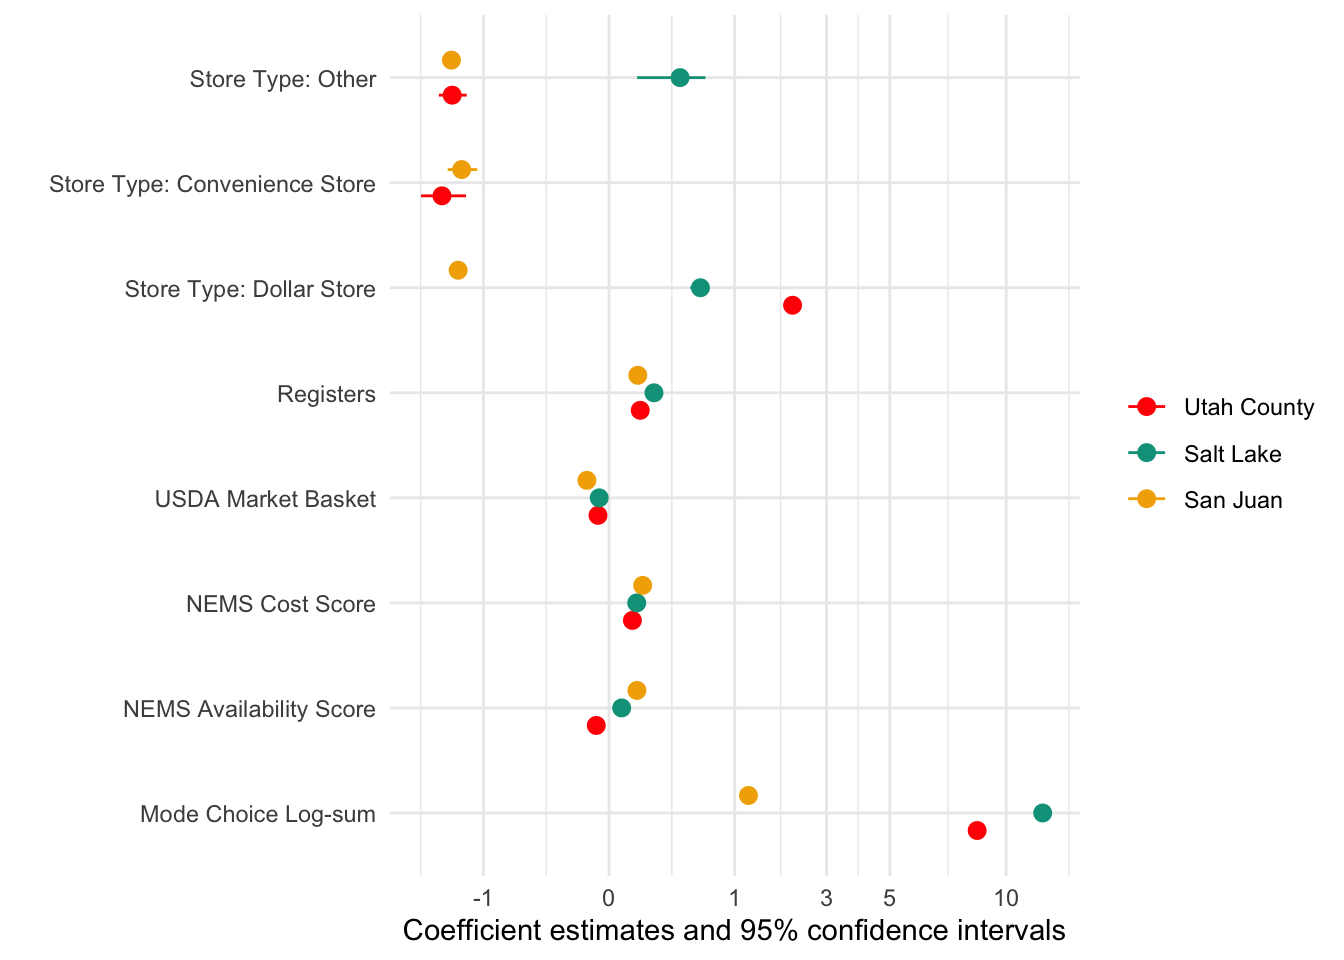
\includegraphics[width=6in,height=\textheight]{04_estimation_files/figure-pdf/fig-all-comp-1.pdf}

}

\caption{\label{fig-all-comp}Comparison of county model coefficient
estimates. Absolute square root transformation applied to improve
visibility.}

\end{figure}%

To better visualize how the preferences in the three communities differ
from each other, Figure~\ref{fig-all-comp} plots the coefficient
estimates from the All model in each community. The mode choice log-sum
is strongly significant in all three communities, but it has its
smallest value in San Juan County where people often must travel long
distances to reach any stores. The highest mode choice log-sum value is
in Salt Lake, but this explains a smaller proportion of the model
outcomes than the lower value in Utah County; a possible hypothesis for
this observation may include the higher density of stores in Salt Lake
--- attributes are more important when so many stores are close together
--- paired with the somewhat lower vehicle ownership in that community
driving up the coefficient value. Most other estimates are somewhat
consistent across counties, with the exception of the NEMS variables
discussed previously and the role of dollar stores and other stores in
each community.

\subsection{Accessibility}\label{sec-access}

With the models estimated in Section~\ref{sec-estimation}, we can
evaluate the spatial access of each community. Figure~\ref{fig-map-ut}
shows the value of the grocery store destination choice log-sum for
block groups in Utah County. Unsurprisingly, the block groups in the
core of the urban areas of the region have the highest access to grocery
stores, because this is where the stores are located and also where the
transportation access to multiple destinations is highest. This map also
contains somewhat interesting implications for the equity of access. A
perhaps unique feature of Utah County's demographic geography is that
the wealthiest neighborhoods tend to be located on the mountain benches
east of the main urban areas. This means that in Utah County, at least,
the neighborhoods with the lowest access to grocery stores are actually
some of the wealthiest neighborhoods with the lowest concentrations of
ethnic minorities in the region.

\begin{figure}

\centering{

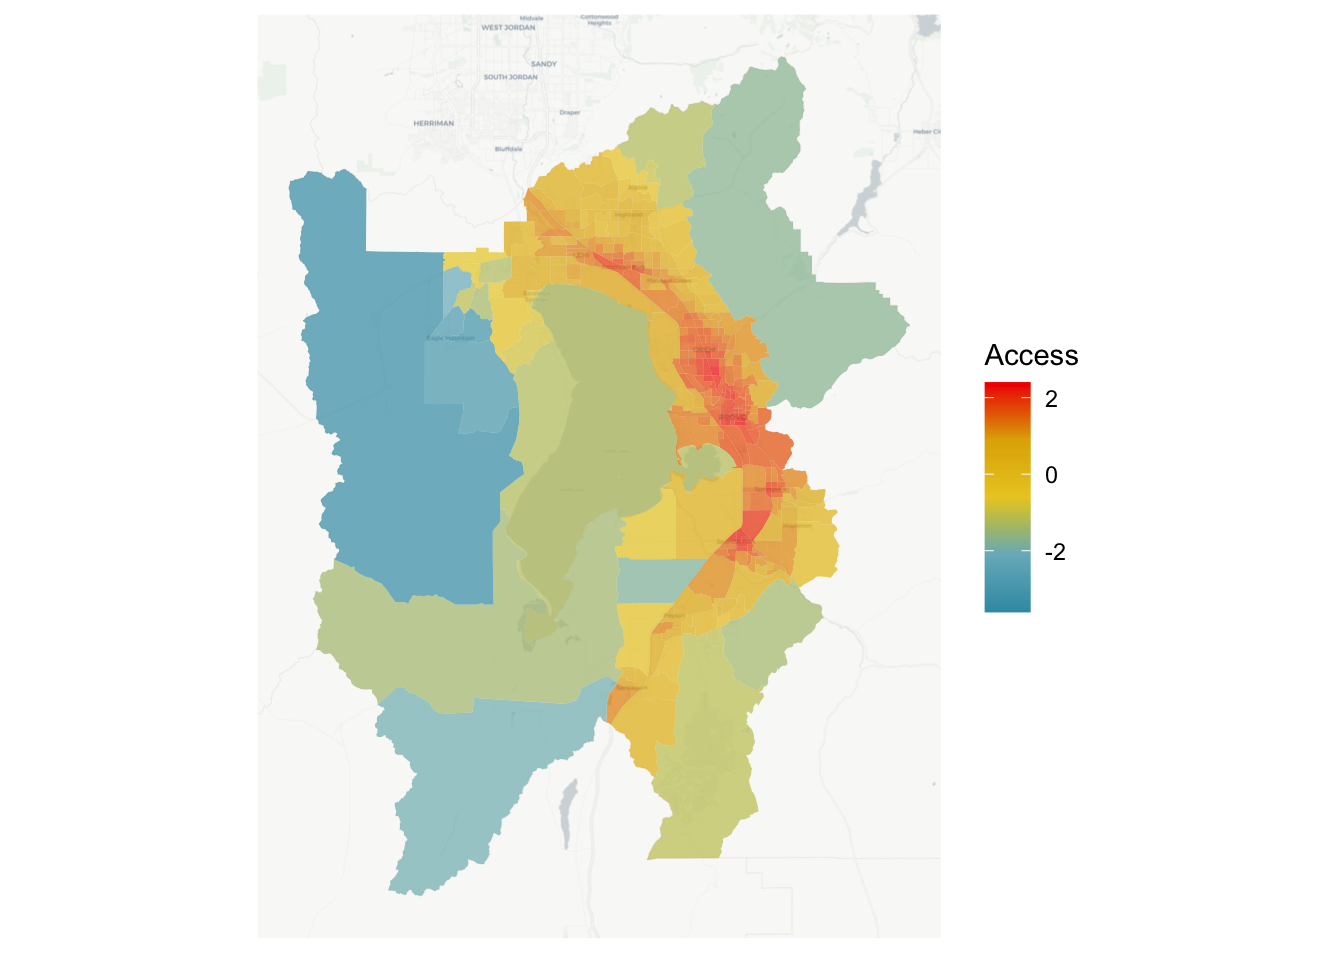
\includegraphics[width=6in,height=\textheight]{04_estimation_files/figure-pdf/fig-map-ut-1.pdf}

}

\caption{\label{fig-map-ut}Modeled access to grocery stores in Utah
County}

\end{figure}%

Of course, much of this high access in the urban core of Utah County is
achieved by cheap and available automobile transportation. We can
consider what access looks like for those without cars by re-computing
the mode choice log-sum described in Section~\ref{sec-mcls} between all
block group / store pairs but eliding the automobile mode, and examining
the resulting impact to destination choice utility.
Figure~\ref{fig-map-nocar} shows the results of this analysis: whereas
the total access (with car included) is a smooth gradient across the
valley, the access for individuals without vehicles is blocky and
discontinuous, with neighborhoods of relatively good access immediately
next to neighborhoods with bad or non-existent access. This may reflect
the discontinuous nature of active transport and public transit
facilities in the region, as well as the auto-dominated locations of
many grocery stores. Note also that even for neighborhoods of relatively
good non-vehicle access, the destination choice log-sum value is
substantially lower than the logsum with vehicle access; the minimum
value on with vehicles is just below 0, whereas the \emph{maximum}
log-sum without vehicles is around -100. Because the log-sum occurs on
the same scale in both cases, this represents a serious additional cost
for non-vehicle users.

\begin{sidewaysfigure}

\begin{minipage}{0.50\linewidth}

\centering{

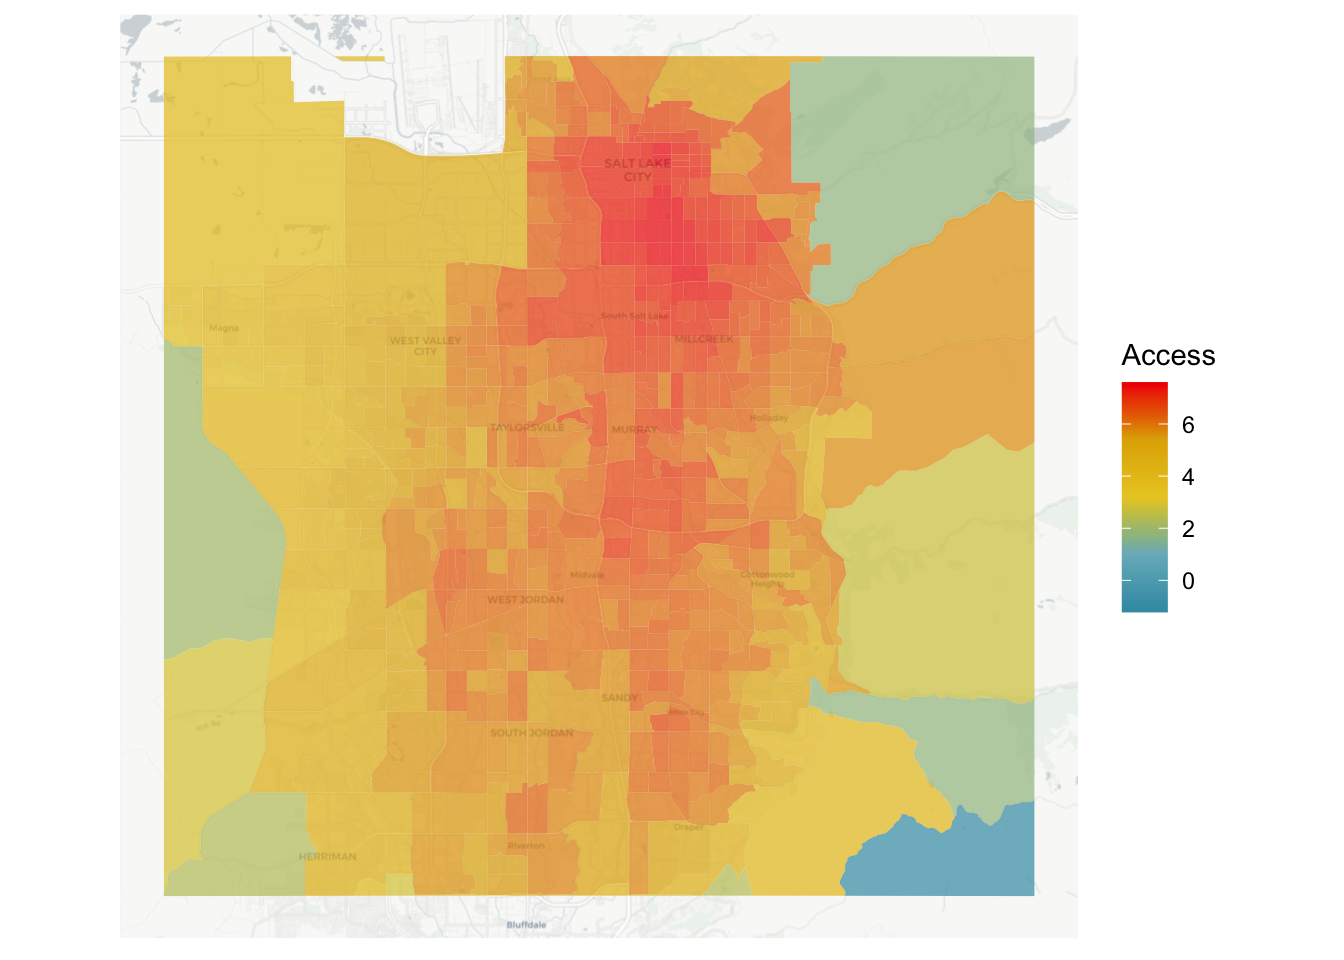
\includegraphics[width=4in,height=\textheight]{04_estimation_files/figure-pdf/fig-map-nocar-1.pdf}

}

\subcaption{\label{fig-map-nocar-1}With vehicles}

\end{minipage}%
%
\begin{minipage}{0.50\linewidth}

\centering{

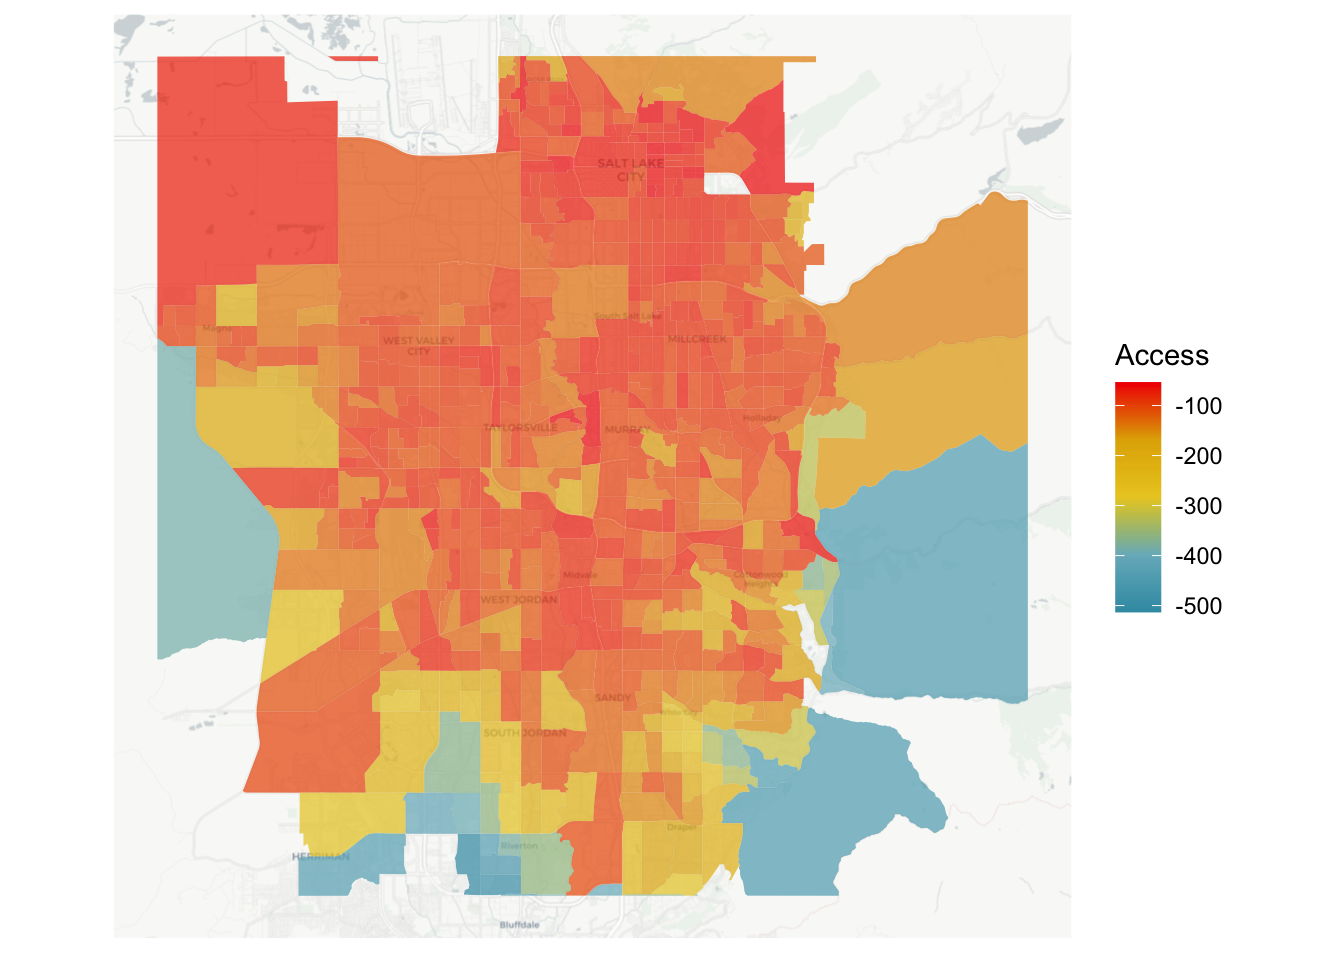
\includegraphics[width=4in,height=\textheight]{04_estimation_files/figure-pdf/fig-map-nocar-2.pdf}

}

\subcaption{\label{fig-map-nocar-2}Without vehicles}

\end{minipage}%

\caption{\label{fig-map-nocar}Access to groceries in Salt Lake County
with and without a vehicle.}

\end{sidewaysfigure}%

\bookmarksetup{startatroot}

\section{Application}\label{sec-scenarios}

In this section, we develop a series of scenarios to which we apply the
models estimated in Section~\ref{sec-results}. These scenarios are
constructed to ascertain what may be the best strategy to improve
nutrition access in a community. We first describe how each scenario was
constructed, and then discuss the results together.

The accessibility of each scenario is determined using the approximated
utility coefficients of the All model estimated in
Section~\ref{sec-results},
\begin{equation}\phantomsection\label{eq-scenu}{
U_{ij}= \beta_{MCLS}( k_{ij}) +  \beta_{n-a} (\mathrm{NEMS-Availability}) +
  \beta_{n-c}\mathrm({NEMS-Cost}) + \\ \beta_{mkt} (\mathrm{Market Basket}) + \pmb{\beta}_{type}(\mathrm{Type})  
}\end{equation} and the total access benefit is defined as the consumer
surplus given in Equation~\ref{eq-cs}. Note that this benefit is
denominated in units of utility (Ben-Akiva \& Lerman, 1985), and the
coefficients in Equation~\ref{eq-scenu} serve to convert between the
units of the variable and utility. Specifically, the \(\beta_{mkt}\)
coefficient represents how many dollars of grocery cost a person is
willing to spend to increase their utility by one unit.

In actuality, the utility formula in Equation~\ref{eq-scenu} is a
relative utility added by an unknown constant,
\(U_{ij} = f(\mathbf{\beta}, X_{ij}) + C\), but this \(C\) term is
included in all the alternatives and therefore cancels out (Train, 2009)
in estimation. This means we cannot assess the \emph{absolute} value of
utility, but we can assess the \emph{relative} monetary benefit of the
difference between two scenarios as \[
\mathrm{Benefit} = \sum_{i}\left(-\frac{\omega_i}{\beta_{mkt}}(CS_i^1 - CS_i^1)\right)
\] where a weight \(\omega\) accounts for the population in each origin
zone \(i\) and the \(\beta_{mkt}\) converts the difference in utility
into a dollar amount.

\subsection{Scenario Descriptions}\label{scenario-descriptions}

There are three general strategies we develop scenarios around:

\begin{enumerate}
\def\labelenumi{\arabic{enumi}.}
\tightlist
\item
  Erect a new grocery store in the community, in a place where one does
  not already exist.
\item
  Improve an existing convenience store or dollar store so that it has
  the attributes of a full-service grocery store.
\item
  Improve the transit and non-motorized access to stores in a region.
\end{enumerate}

We implement all three strategies in scenarios on the west Salt Lake
valley community. We also implement strategy 1 (a new store) in the San
Juan and Utah County communities for comparison.

\subsubsection{Erect a new store}\label{erect-a-new-store}

This strategy assumes that the nutrition environment would benefit from
a new store located in a place that presently has low grocery store
access. To examine the potential for this strategy to improve access to
nutrition in each community, we calculate the change in destination
choice log-sum when a new store is added to the region in a location
where access is currently poor. The new store is a full-service grocery
store with a number of registers equal to the mean of other grocery
stores in the community, and NEMS availability score, NEMS cost score,
and market basket cost equivalent to the 75\(^{th}\) percentile for the
community. Thus the store is expected to be better-than-average quality
as perceived by the residents of the community. The location for this
new store is at 4100 S and 2700 W in West Valley City.

\subsubsection{Improve an existing
store}\label{improve-an-existing-store}

This strategy assumes that existing stores are in locations that the
community values and can access, but that those stores may not have high
availability of quality goods. To examine the potential for this
strategy to improve access to nutrition, we improve the attributes of an
existing dollar store in the community so that it has the size, prices,
and availability of goods as a full-service grocery store. As above, we
create a full-service grocery store with a number of registers equal to
the mean of other grocery stores in the community, and NEMS availability
score, NEMS cost score, and market basket cost equivalent to the
75\(^{th}\) percentile for the community. Thus the store is expected to
be better-than-average quality as perceived by the residents of the
community; the difference from the previous scenario is that the
improved store takes the place of an existing convenience store or
dollar store.

The improved stores are at the following locations in each community:

\begin{itemize}
\tightlist
\item
  An ethnic store near 2700 W 3500 S in West Valley City (Salt Lake)
\item
  A small grocery store in Santaquin (Utah County)
\item
  A dollar store in Blanding (San Juan County)
\end{itemize}

\subsubsection{Improve transit and non-motorized
transport}\label{improve-transit-and-non-motorized-transport}

This strategy assumes that people cannot easily travel to existing
stores because they cannot or do not drive for a variety of reasons, and
that the public and active transport networks provide an insufficient
level of service. To examine the potential for this strategy to improve
access to nutrition, we improve the travel time costs in the Salt Lake
community for non-motorized and public transportation in the region and
calculate the change in destination choice log-sum.

For active transportation, the lack of pedestrian facilities across and
alongside roads both in reality and in the OpenStreetMap dataset may
substantially increase measured walk distances and times. In this
scenario, we replace the times measured from OpenStreetMap using R5 with
an idealized Euclidean distance function,
\begin{equation}\phantomsection\label{eq-newwalk}{
t_{\mathrm{walk}} = \frac{\sqrt{2} * d'_{ij}}{v_{\mathrm{walk}}}
}\end{equation} where \(d'_{ij}\) is the Euclidean (straight-line)
distance between \(i\) and \(j\) and \(v_{ij}\) is an average walking
speed equivalent to 3.5 feet per second (Fitzpatrick et al., 2006). The
distance is multiplied by the square root of 2 to reflect the Manhattan
distance (along a gridded street system). We retain the cap on walking
distance at 10 kilometers. Though this distance may radically understate
the real walking distance, we are trying to create an idealized scenario
of effectively frictionless active transport. For public transit, we
assume that the frequency of service is such that all transfer and
initial wait times are at most 5 minutes, and that no person must walk
more than 10 minutes to access their first public transport service.

Travel times are improved in this way for all block group --- store
pairs in the west Salt Lake Valley community.

\subsection{Scenario Results}\label{scenario-results}

Using the methodology described above, we recalculated the destination
choice log-sum value for each block group under each scenario, and
compared the change in accessibility resulting from the improvement.

\begin{figure}

\centering{

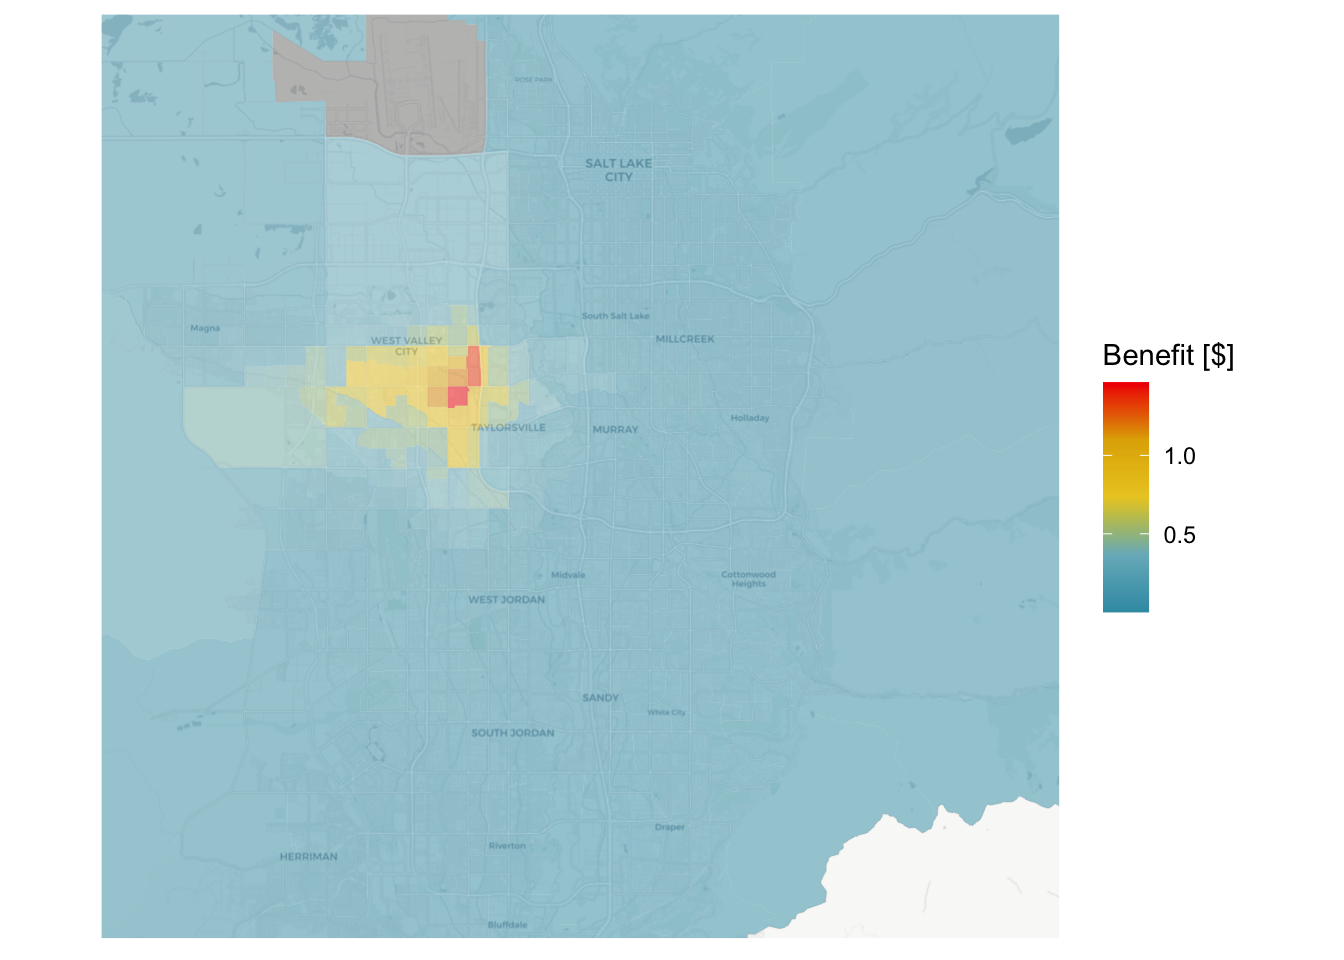
\includegraphics[width=6in,height=\textheight]{05_scenarios_files/figure-pdf/fig-s1results-1.pdf}

}

\caption{\label{fig-s1results}Estimated per-household benefits of adding
new full-service store in west Salt Lake Valley}

\end{figure}%

Figure~\ref{fig-s1results} shows the geographic distribution of benefits
associated with locating a new store at a site in the Salt Lake
community. The benefits are largest immediately next to the new store,
where they exceed \(317\) for each household each time the household
makes a trip to a grocery store.

\begin{figure}

\centering{

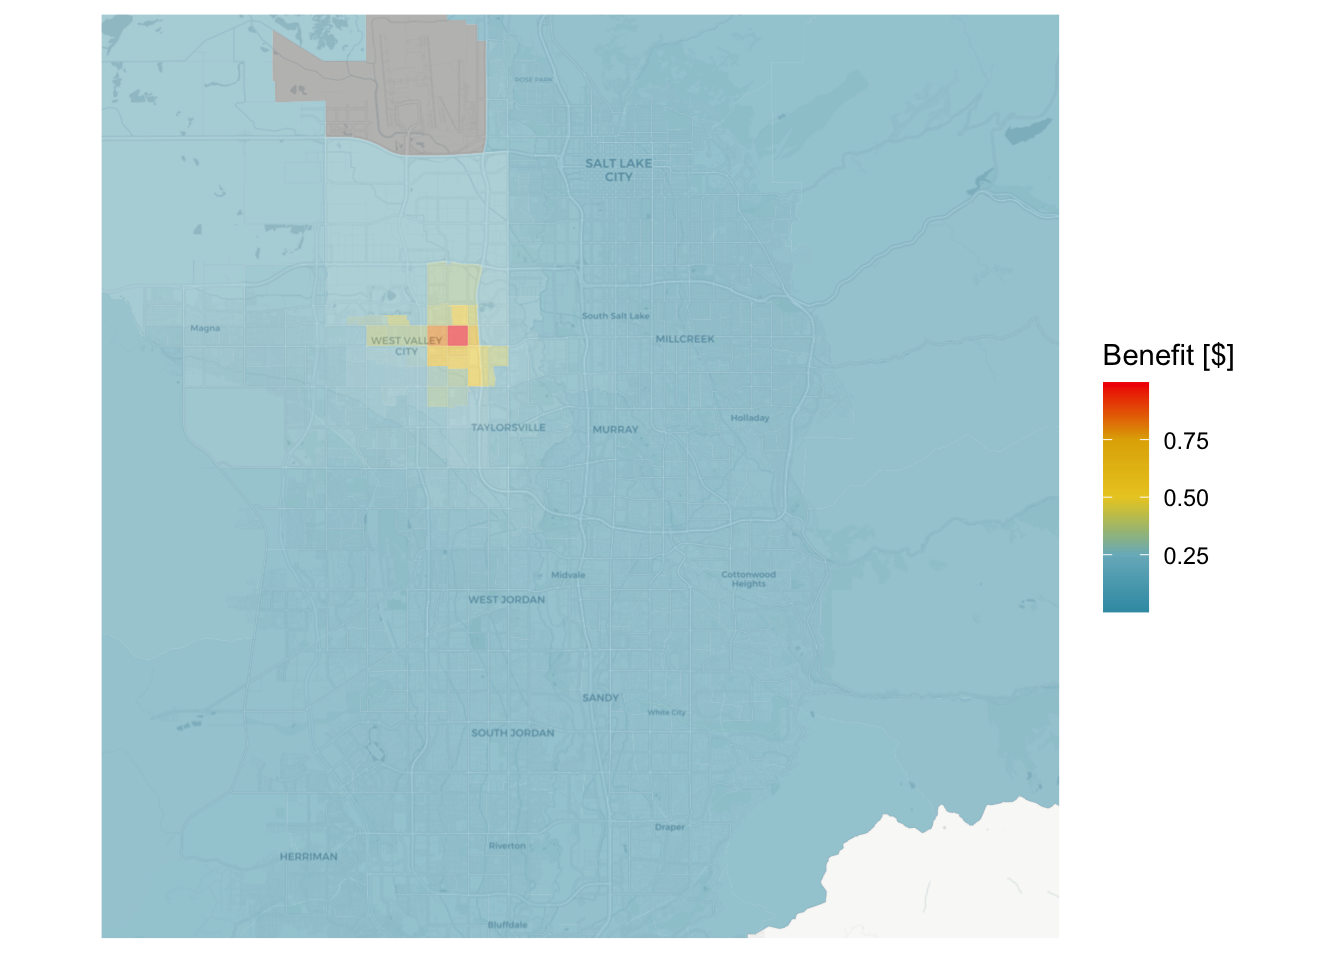
\includegraphics[width=6in,height=\textheight]{05_scenarios_files/figure-pdf/fig-s2results-1.pdf}

}

\caption{\label{fig-s2results}Estimated per-household benefits of
improving an existing store in west Salt Lake Valley}

\end{figure}%

Figure~\ref{fig-s2results} shows the results of the scenario improving
an existing store in the Salt Lake community. Compared to the results of
the new store scenario, the scale of the benefits are not as substantial
(a maximum per-household-trip benefit of less than \$1), and seem to not
cover quite as large a geographic region. Figure~\ref{fig-s2sjut} shows
the results of improving a store in Utah and San Juan Counties. As in
Salt Lake, the benefits are most strongly concentrated in the immediate
vicinity of the improved store. One interesting observation ---
especially in Utah County --- is that the improvements are felt more
strongly in the block groups near the improved store that have lower
availability of other options. The block group in Utah County directly
containing the improvement sees a per-household-trip benefit well over
\$2, considerably more than the maximum benefit in Salt Lake. This is
intuitive, as the improvement of a store matters less if the stores
close to you are already sufficient.

\begin{figure}

\begin{minipage}{0.50\linewidth}

\centering{

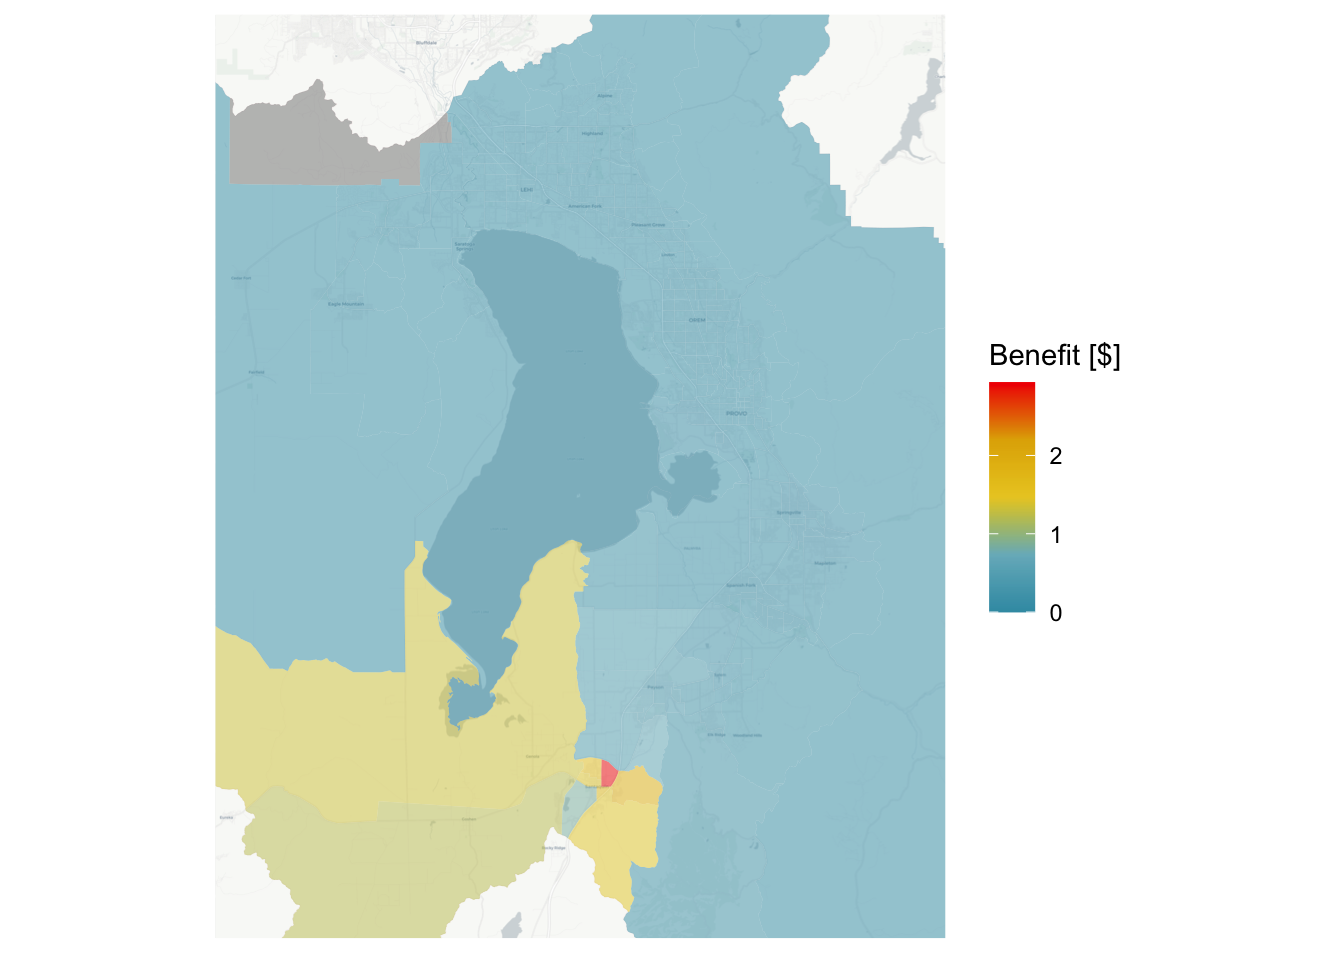
\includegraphics[width=4in,height=\textheight]{05_scenarios_files/figure-pdf/fig-s2sjut-1.pdf}

}

\subcaption{\label{fig-s2sjut-1}Utah County (in Santaquin)}

\end{minipage}%
%
\begin{minipage}{0.50\linewidth}

\centering{

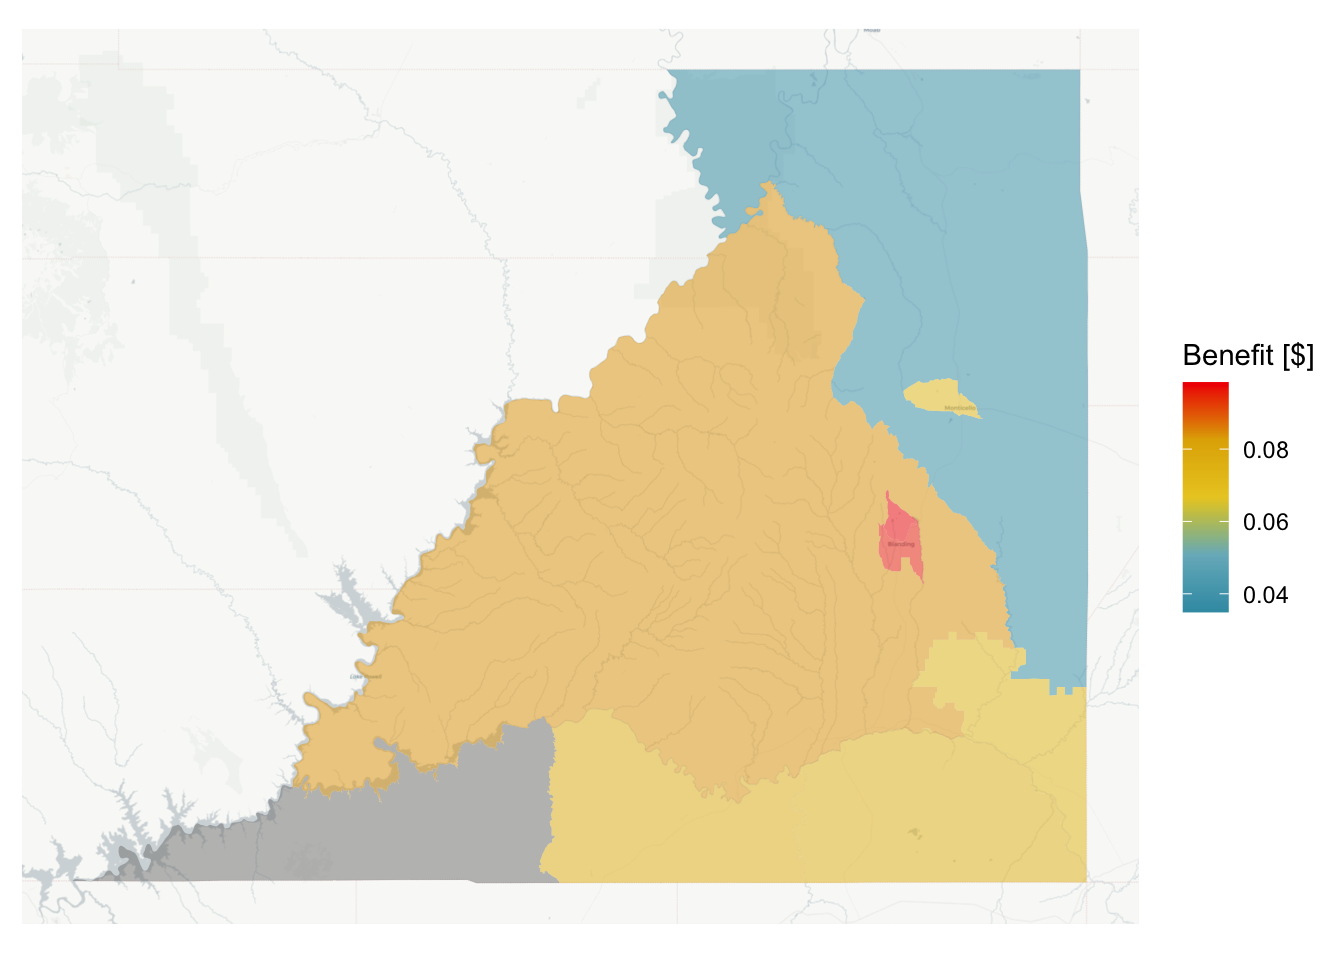
\includegraphics[width=4in,height=\textheight]{05_scenarios_files/figure-pdf/fig-s2sjut-2.pdf}

}

\subcaption{\label{fig-s2sjut-2}San Juan County (in Blanding)}

\end{minipage}%

\caption{\label{fig-s2sjut}Estimated per-household benefits of improving
an existing store in Utah and San Juan Counties.}

\end{figure}%

The results of the third scenario, improving the access of non-motorized
and public transit access to stores, are shown in
Figure~\ref{fig-s3results}. This benefit is spread over a larger area,
and is concentrated on the 35 MAX bus rapid transit corridor where the
improvement in walk access time to transit couples with high frequency
transit service to large grocery stores on the corridor. The
per-household-trip benefit is very small however, with a maximum benefit
on the order of \$0.25.

\begin{figure}

\centering{

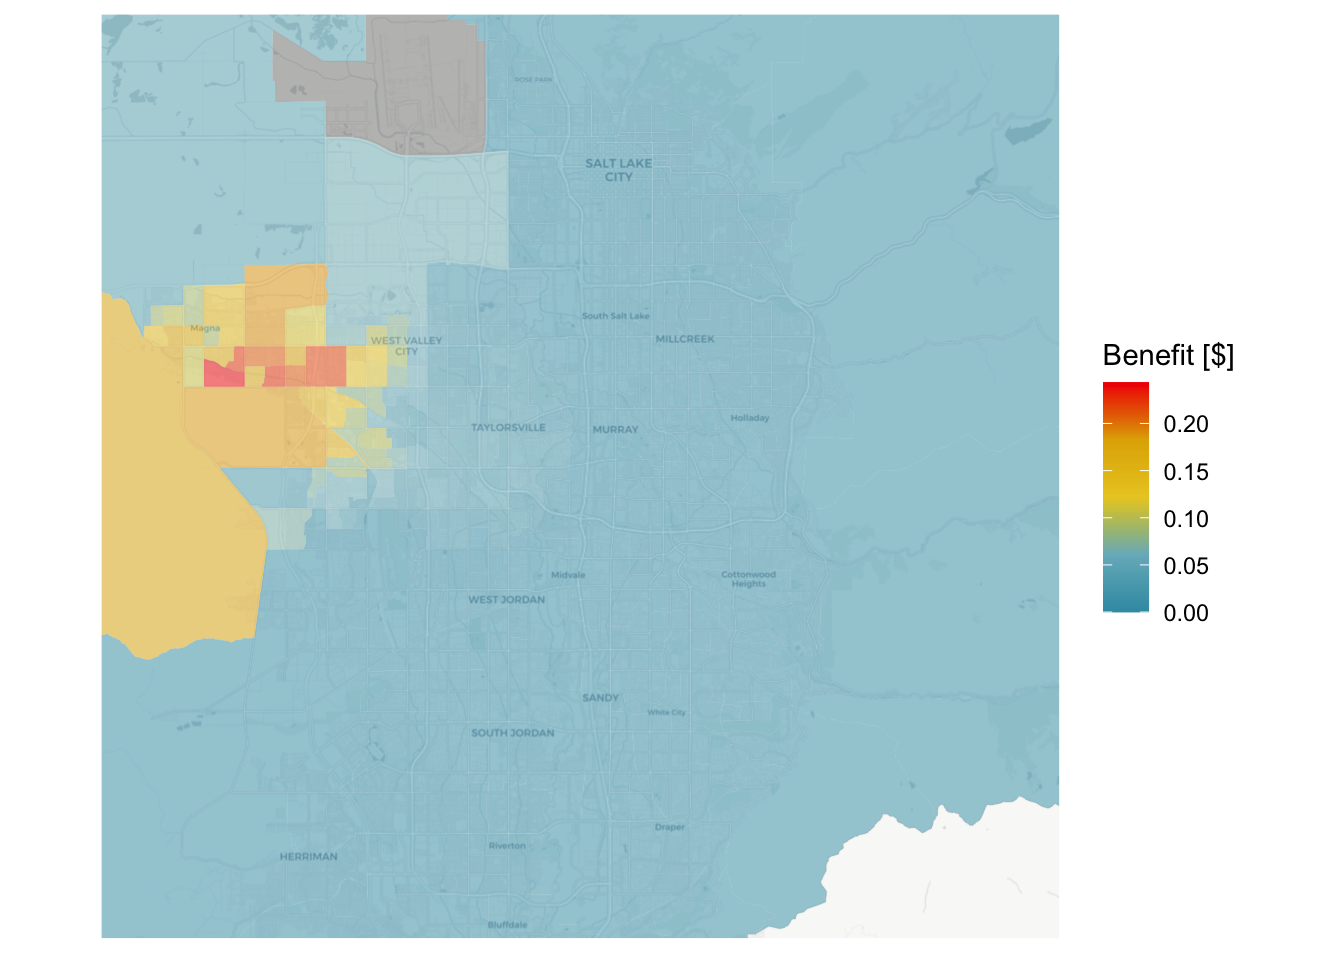
\includegraphics[width=6in,height=\textheight]{05_scenarios_files/figure-pdf/fig-s3results-1.pdf}

}

\caption{\label{fig-s3results}Estimated per-household benefits of
improving non-motorized and public transport access to groceries in Salt
Lake Valley.}

\end{figure}%

\begin{table}

\caption{\label{tbl-scenarios}Scenario Benefits}

\centering{

\centering
\begin{tabular}[t]{llll}
\toprule
\multicolumn{1}{c}{ } & \multicolumn{3}{c}{Weighted by} \\
\cmidrule(l{3pt}r{3pt}){2-4}
Scenario & Households & Non-white & Low-Income\\
\midrule
New Store & \$11,145,542,384 & \$3,051,365,881 & \$1,766,485,839\\
\addlinespace[0.3em]
\multicolumn{4}{l}{\textbf{Improved Store}}\\
\hspace{1em}Salt Lake Valley & \$8,597,772 & \$4,187,114 & \$1,760,422\\
\hspace{1em}Utah County & \$1,621,027 & \$260,360 & \$249,142\\
\hspace{1em}San Juan County & \$355,512 & \$157,715 & \$114,897\\
Improved Transport & \$2,024,639 & \$922,766 & \$287,064\\
\bottomrule
\end{tabular}

}

\end{table}%

Although comparing the geographic distribution of benefits is helpful,
the aggregate benefit is more likely to guide policy. Additionally, the
aggregate benefits can be weighted in different ways to understand the
effects of the various policies on different populations.
Table~\ref{tbl-scenarios} presents the aggregate benefit from each of
the three scenarios (and the result of the second scenario in all three
communities). The Households column multiplies the difference in
destination choice log-sum at each block group by the number of
households in that block group, while the non-white and low-income
columns weight the difference by the share of non-white individuals and
low-income households respectively. All demographic data comes from the
American Community Survey 5-year aggregations.

These alternate weighting schemes help to illustrate the potential
equity of the benefit distribution should each scenario be pursued. The
new store scenario in the Salt Lake community, for example, has a total
benefit of approximately \$5.5 million. Of this amount, somewhat less
than half the benefits go to non-white individuals and less than
one-fifth to low-income households. These ratios are more or less the
same for the store improvement scenario and the improved transport
scenario in the Salt Lake Valley. The Utah County store improvement, on
the other hand, has a somewhat higher proportion of benefits going to
low-income households relative to non-white households. This is a
reflection of the lower minority population in southern Utah County vis
a vis west Salt Lake valley, but is nonetheless a metric that program
evaluators might pay attention to.

Overall, the improved store brings more than twice the benefits of
improving non-automobile transportation, and the new store more than
five times the benefits. Understanding the costs of these various
alternatives is outside the scope of this research, but the level of
infrastructure investment required to increase transportation level of
service to that constructed in the simulation is likely an order of
magnitude higher than the cost of a single new grocery store. It should
also be acknowledged that improving non-automobile infrastructure and
services would have benefits beyond just grocery store trips that we do
not attempt to enumerate here. It is also not clear whether the level of
improvement simulated in the second scenario could be accomplished
within the envelope of the existing store; it may be that such
improvements would meet or exceed the cost of building a new store on a
new site, along with stocking, staffing, and operating the store.

\bookmarksetup{startatroot}

\section{Conclusions and Recommendations}\label{sec-conclude}

Access to nutrition is a critical topic that has been a frequent focus
of academic literature in public health, community planning, and
engineering, but the varying and incomplete quantitative definitions of
access have perhaps limited efforts at developing solutions.

In this research, the model we developed and informed with
location-based services data suggested that policies that increased the
availability and quality of grocery stores would do more to enhance
access to nutrition than strategies that increased the transit level of
service and lowered active transport travel times in three different
Utah communities. These findings may not be general, but they largely
support the review of food desert literature in (Beaulac et al., 2009)
as well as critical evaluations by (Shannon, 2014) and (Wright et al.,
2016).

\subsection{Limitations}\label{sec-limitations}

A number of assumptions made in Section~\ref{sec-methods} lead to
limitations that other reasonable researchers might pursue differently,
and thereby obtain marginally different outcomes.

In selecting a survey instrument with which to collect the store
attribute data, we selected an existing and validated instrument from
the nutrition environment literature. The NEMS-S focus on low-calorie
and low-fat alternatives may be somewhat outdated in view of modern
nutritional guidelines. For example, the NEMS-S does not track the
availability and price of poultry, as ``lean'' poultry is not a goods
category in the way that ground beef comes with multiple fat contents.
Thus a major source of protein in typical American diets (FNS, 2021) was
not traced across stores in each community. On a more basic level, the
NEMS-S attempts to measure a store's stocking of goods that researchers
believe are beneficial, and does not measure either what people wish to
buy, or what they are actually buying at a store. Future research might
attempt to survey shoppers on what they actually purchased at each store
--- or collect receipts of their purchases --- though this would
substantially raise the difficulty of collecting data.

Most households do not obtain all their groceries at a single store,
though this research of necessity assumed that a simulated person chose
exactly one store from stores available to them. Similarly, the
location-based services data provided by StreetLight and used to
identify which stores people traveled to only reveal whether a device
was identified inside a geographic polygon, and not what they were
actually doing in that polygon. This research had no way of
distinguishing, for example, whether an individual device observed at a
dollar store or a super market (e.g.~Wal-Mart) was there to purchase
groceries or some other household goods that might not be offered at
more traditional food markets.

A number of simplifying assumptions concern the socioeconomic and
spatio-temporal detail supplied to the choice models and accessibility
calculators. The StreetLight data do not contain any demographic
information on the individuals making trips, beyond the inferences made
possible by the residence block group. This makes it difficult to
estimate whether lower income households are more or less sensitive to
travel distances or prices. Additionally, the research assumed that
every trip was from the population-weighted block group centroid, which
may vary substantially from the actual distance traveled, especially in
large block groups. The methodology also used travel times calculated in
the AM peak hour; though this time maximizes the availability of transit
options, it is not a typical peak time for grocery shopping. All of
these limitations could potentially be relaxed by using a synthetic
population with detailed socioeconomic data and parcel-level locations
determined by an activity-based model, as proposed by (Dong et al.,
2006). In this exercise, which we leave to future research, the grocery
maintenance trips could be explicitly modeled, with synthetic
individuals of unique characteristics choosing destinations that are
available on the course of their other daily activities, using their
chosen travel modes. This proposal would effectively extend the methods
of (Widener \& Shannon, 2014) within the framework of explicit
activity-travel modeling.

Finally, the scenarios presented in Section~\ref{sec-scenarios} are
designed to illustrate potential applications of this accessibility
methodology, with a comparative analysis of strategies to improve access
to nutrition. Selecting different sites, attribute levels, or transport
policies might substantially change the scale or rank-ordering of the
estimated benefits. A comprehensive search for the location that would
maximize benefits would be an interesting exercise, which we also leave
to future research.

\bookmarksetup{startatroot}

\section*{Acknowledgments}\label{acknowledgments}
\addcontentsline{toc}{section}{Acknowledgments}

\markboth{Acknowledgments}{Acknowledgments}

The authors acknowledge the Utah Department of Transportation (UDOT) for
funding this research. The authors alone are responsible for the
preparation and accuracy of the information, data, analysis,
discussions, recommendations, and conclusions presented herein. The
contents do not necessarily reflect the views, opinions, endorsements,
or policies of the Utah Department of Transportation or the U.S.
Department of Transportation. The Utah Department of Transportation
makes no representation or warranty of any kind, and assumes no
liability therefore.

Student research assistants who collected the store data include Kaeli
Monahan, Brooke Jones, Emily Aleson, Andrea Barney, Mattie Earnest, Tare
Ekpagha, Mackay Graper, Olivia Harrison, Mary Jacobsen, Gillian Martin,
Maggie Plessinger, and Jenna Smith. Madeleine Smith coordinated the data
collection efforts.

Graphics in the document are produced with multiple R packages
(Arel-Bundock, 2022; Dunnington, 2023; Ram \& Wickham, 2018; Wickham,
2016).

\subsection*{Author Contribution
Statement}\label{author-contribution-statement}
\addcontentsline{toc}{subsection}{Author Contribution Statement}

\markright{Author Contribution Statement}

\textbf{Gregory S. Macfarlane:} Conceptualization, Methodology,
Software, Resources, Writing - original draft, Visualization,
Supervision \textbf{Emma Stucki:} Software, Investigation, Data
curation, Writing - original draft \textbf{Myrranda Salmon:}
Investigation, Data curation \textbf{Alisha H. Redelfs:} Methodology,
Resources, Writing - review \& editing \textbf{Lori Spruance:}
Methodology, Resources, Writing - review \& editing

\bookmarksetup{startatroot}

\section*{References}\label{references}
\addcontentsline{toc}{section}{References}

\markboth{References}{References}

\phantomsection\label{refs}
\begin{CSLReferences}{1}{0}
\bibitem[\citeproctext]{ref-modelsummary}
Arel-Bundock, V. (2022). {modelsummary}: Data and model summaries in
{R}. \emph{Journal of Statistical Software}, \emph{103}(1), 1--23.
\url{https://doi.org/10.18637/jss.v103.i01}

\bibitem[\citeproctext]{ref-barnes2021}
Barnes, M. (2021). \emph{Resiliency of {Utah}'s {Road Network}: {A
Logit-Based Approach}} {[}\{\{MS Thesis\}\}{]}. Brigham Young
University.

\bibitem[\citeproctext]{ref-beaulac2009}
Beaulac, J., Kristjansson, E., \& Cummins, S. (2009).
\href{https://www.ncbi.nlm.nih.gov/pmc/articles/PMC2722409}{A
{Systematic Review} of {Food Deserts}, 1966-2007}. \emph{Preventing
Chronic Disease}, \emph{6}(3), A105.

\bibitem[\citeproctext]{ref-ben-akiva1985}
Ben-Akiva, M., \& Lerman, S. R. (1985). \emph{Discrete {Choice
Analysis}: {Theory} and {Applications} to {Travel Demand}}. MIT Press.
\url{https://www.jstor.org/stable/1391567}

\bibitem[\citeproctext]{ref-bureauoflaborstatistics2023}
Bureau of Labor Statistics. (2023). 12-month percentage change,
{Consumer Price Index}, selected categories. In \emph{Consumer Price
Index}.
https://www.bls.gov/charts/consumer-price-index/consumer-price-index-by-category-line-chart.htm.

\bibitem[\citeproctext]{ref-chen2016}
Chen, D., Jaenicke, E. C., \& Volpe, R. J. (2016). Food {Environments}
and {Obesity}: {Household Diet Expenditure Versus Food Deserts}.
\emph{American Journal of Public Health}, \emph{106}(5), 881--888.
\url{https://doi.org/10.2105/AJPH.2016.303048}

\bibitem[\citeproctext]{ref-clifton2004}
Clifton, K. J. (2004). Mobility {Strategies} and {Food Shopping} for
{Low-Income Families}: {A Case Study}. \emph{Journal of Planning
Education and Research}, \emph{23}(4), 402--413.
\url{https://doi.org/10.1177/0739456X04264919}

\bibitem[\citeproctext]{ref-conway2018}
Conway, M. W., Byrd, A., \& Eggermond, M. van. (2018). Accounting for
uncertainty and variation in accessibility metrics for public transport
sketch planning. \emph{Journal of Transport and Land Use}, \emph{11}(1).
\url{https://doi.org/10.5198/jtlu.2018.1074}

\bibitem[\citeproctext]{ref-conway2017}
Conway, M. W., Byrd, A., \& van der Linden, M. (2017). Evidence-{Based
Transit} and {Land Use Sketch Planning Using Interactive Accessibility
Methods} on {Combined Schedule} and {Headway-Based Networks}.
\emph{Transportation Research Record}, \emph{2653}(1), 45--53.
\url{https://doi.org/10.3141/2653-06}

\bibitem[\citeproctext]{ref-conway2019}
Conway, M. W., \& Stewart, A. F. (2019). Getting {Charlie} off the
{MTA}: A multiobjective optimization method to account for cost
constraints in public transit accessibility metrics. \emph{International
Journal of Geographical Information Science}, \emph{33}(9), 1759--1787.
\url{https://doi.org/10.1080/13658816.2019.1605075}

\bibitem[\citeproctext]{ref-cooksey-stowers2017}
Cooksey-Stowers, K., Schwartz, M. B., \& Brownell, K. D. (2017). Food
{Swamps Predict Obesity Rates Better Than Food Deserts} in the {United
States}. \emph{International Journal of Environmental Research and
Public Health}, \emph{14}(11), 1366.
\url{https://doi.org/10.3390/ijerph14111366}

\bibitem[\citeproctext]{ref-mlogit}
Croissant, Y. (2020). Estimation of random utility models in {R}: The
{mlogit} package. \emph{Journal of Statistical Software}, \emph{95}(11),
1--41. \url{https://doi.org/10.18637/jss.v095.i11}

\bibitem[\citeproctext]{ref-dong2006}
Dong, X., Ben-Akiva, M. E., Bowman, J. L., \& Walker, J. L. (2006).
Moving from trip-based to activity-based measures of accessibility.
\emph{Transportation Research Part A: Policy and Practice},
\emph{40}(2), 163--180. \url{https://doi.org/10.1016/j.tra.2005.05.002}

\bibitem[\citeproctext]{ref-ggspatial}
Dunnington, D. (2023). \emph{Ggspatial: Spatial data framework for
ggplot2}. \url{https://CRAN.R-project.org/package=ggspatial}

\bibitem[\citeproctext]{ref-fitzpatrick2006}
Fitzpatrick, K., Brewer, M. A., \& Turner, S. (2006). Another {Look} at
{Pedestrian Walking Speed}. \emph{Transportation Research Record},
\emph{1982}(1), 21--29.
\url{https://doi.org/10.1177/0361198106198200104}

\bibitem[\citeproctext]{ref-fns2021}
FNS. (2021). \emph{Thrifty {Food Plan}}. {Food and Nutrition Service,
United States Department of Agriculture}.

\bibitem[\citeproctext]{ref-geurs2010}
Geurs, K., Zondag, B., de Jong, G., \& de Bok, M. (2010). Accessibility
appraisal of land-use/transport policy strategies: {More} than just
adding up travel-time savings. \emph{Transportation Research Part D:
Transport and Environment}, \emph{15}(7), 382--393.
\url{https://doi.org/10.1016/j.trd.2010.04.006}

\bibitem[\citeproctext]{ref-ghosh-dastidar2014}
Ghosh-Dastidar, B., Cohen, D., Hunter, G., Zenk, S. N., Huang, C.,
Beckman, R., \& Dubowitz, T. (2014). Distance to {Store}, {Food Prices},
and {Obesity} in {Urban Food Deserts}. \emph{American Journal of
Preventive Medicine}, \emph{47}(5), 587--595.
\url{https://doi.org/10.1016/j.amepre.2014.07.005}

\bibitem[\citeproctext]{ref-glanz2007}
Glanz, K., Sallis, J. F., Saelens, B. E., \& Frank, L. D. (2007).
Nutrition {Environment Measures Survey} in {Stores} ({NEMS-S}):
{Development} and {Evaluation}. \emph{American Journal of Preventive
Medicine}, \emph{32}(4), 282--289.
\url{https://doi.org/10.1016/j.amepre.2006.12.019}

\bibitem[\citeproctext]{ref-handy1997}
Handy, S. L., \& Niemeier, D. A. (1997). Measuring accessibility: {An}
exploration of issues and alternatives. \emph{Environment and Planning
A: Economy and Space}, \emph{29}(7), 1175--1194.
\url{https://doi.org/10.1068/a291175}

\bibitem[\citeproctext]{ref-hedrick2022}
Hedrick, V. E., Farris, A. R., Houghtaling, B., Mann, G., \& Misyak, S.
A. (2022). Validity of a {Market Basket Assessment Tool} for {Use} in
{Supplemental Nutrition Assistance Program Education Healthy Retail
Initiatives}. \emph{Journal of Nutrition Education and Behavior},
\emph{54}(8), 776--783. \url{https://doi.org/10.1016/j.jneb.2022.02.018}

\bibitem[\citeproctext]{ref-hillier2011}
Hillier, A., Cannuscio, C. C., Karpyn, A., McLaughlin, J., Chilton, M.,
\& Glanz, K. (2011). How {Far Do Low-Income Parents Travel} to {Shop}
for {Food}? {Empirical Evidence} from {Two Urban Neighborhoods}.
\emph{Urban Geography}, \emph{32}(5), 712--729.
\url{https://doi.org/10.2747/0272-3638.32.5.712}

\bibitem[\citeproctext]{ref-kaczynski2016}
Kaczynski, A. T., Schipperijn, J., Hipp, J. A., Besenyi, G. M., Wilhelm
Stanis, S. A., Hughey, S. M., \& Wilcox, S. (2016). {ParkIndex}:
{Development} of a standardized metric of park access for research and
planning. \emph{Preventive Medicine}, \emph{87}, 110--114.
\url{https://doi.org/10.1016/j.ypmed.2016.02.012}

\bibitem[\citeproctext]{ref-liu2022}
Liu, B., Widener, M. J., Smith, L. G., Farber, S., Minaker, L. M.,
Patterson, Z., Larsen, K., \& Gilliland, J. (2022). Disentangling {Time
Use}, {Food Environment}, and {Food Behaviors Using Multi-Channel
Sequence Analysis}. \emph{Geographical Analysis}, \emph{54}(4),
881--917. \url{https://doi.org/10.1111/gean.12305}

\bibitem[\citeproctext]{ref-logan2019}
Logan, T., Williams, T., Nisbet, A., Liberman, K., Zuo, C., \& Guikema,
S. (2019). Evaluating urban accessibility: Leveraging open-source data
and analytics to overcome existing limitations. \emph{Environment and
Planning B: Urban Analytics and City Science}, \emph{46}(5), 897--913.
\url{https://doi.org/10.1177/2399808317736528}

\bibitem[\citeproctext]{ref-lunsford2021}
Lunsford, J., Brunt, A., Foote, J., Rhee, Y., Strand, M., \& Segall, M.
(2021). Analysis of {Availability}, {Quality}, and {Price} of {Food
Options} in {Denver}, {CO Grocery Stores}. \emph{Journal of Hunger \&
Environmental Nutrition}, \emph{16}(3), 297--303.
\url{https://doi.org/10.1080/19320248.2020.1741482}

\bibitem[\citeproctext]{ref-macfarlane2022a}
Macfarlane, G., Voulgaris, C. T., \& Tapia, T. (2022). City parks and
slow streets: {A} utility-based access and equity analysis.
\emph{Journal of Transport and Land Use}, \emph{15}(1), 587--612.
\url{https://doi.org/10.5198/jtlu.2022.2009}

\bibitem[\citeproctext]{ref-mcfadden1974}
McFadden, D. (1974). Conditional logit analysis of qualitative choice
behavior. In P. Zarembka (Ed.), \emph{Frontiers in {Econometrics}} (pp.
105--142). Academic Press.

\bibitem[\citeproctext]{ref-pereira2021}
Pereira, R. H. M., Saraiva, M., Herszenhut, D., Braga, C. K. V., \&
Conway, M. W. (2021). R5r: {Rapid Realistic Routing} on {Multimodal
Transport Networks} with {R}{\textsuperscript{5}} in {R}.
\emph{Findings}. \url{https://doi.org/10.32866/001c.21262}

\bibitem[\citeproctext]{ref-wesanderson}
Ram, K., \& Wickham, H. (2018). \emph{Wesanderson: A wes anderson
palette generator}. \url{https://CRAN.R-project.org/package=wesanderson}

\bibitem[\citeproctext]{ref-recker1978}
Recker, W. W., \& Kostyniuk, L. P. (1978). Factors influencing
destination choice for the urban grocery shopping trip.
\emph{Transportation}, \emph{7}(1), 19--33.
\url{https://doi.org/10.1007/BF00148369}

\bibitem[\citeproctext]{ref-shannon2014}
Shannon, J. (2014). Food deserts: {Governing} obesity in the neoliberal
city. \emph{Progress in Human Geography}, \emph{38}(2), 248--266.
\url{https://doi.org/10.1177/0309132513484378}

\bibitem[\citeproctext]{ref-train2009}
Train, K. E. (2009). \emph{Discrete {Choice Methods} with {Simulation}}
(2nd edition). Cambridge University Press.

\bibitem[\citeproctext]{ref-mice}
van Buuren, S., \& Groothuis-Oudshoorn, K. (2011). {mice}: Multivariate
imputation by chained equations in r. \emph{Journal of Statistical
Software}, \emph{45}(3), 1--67.
\url{https://doi.org/10.18637/jss.v045.i03}

\bibitem[\citeproctext]{ref-walker2010}
Walker, R. E., Keane, C. R., \& Burke, J. G. (2010). Disparities and
access to healthy food in the {United States}: {A} review of food
deserts literature. \emph{Health \& Place}, \emph{16}(5), 876--884.
\url{https://doi.org/10.1016/j.healthplace.2010.04.013}

\bibitem[\citeproctext]{ref-ggplot2}
Wickham, H. (2016). \emph{ggplot2: Elegant graphics for data analysis}.
Springer-Verlag New York. \url{https://ggplot2.tidyverse.org}

\bibitem[\citeproctext]{ref-widener2014}
Widener, M. J., \& Shannon, J. (2014). When are food deserts?
{Integrating} time into research on food accessibility. \emph{Health \&
Place}, \emph{30}, 1--3.
\url{https://doi.org/10.1016/j.healthplace.2014.07.011}

\bibitem[\citeproctext]{ref-wright2016}
Wright, J. D., Donley, A. M., Gualtieri, M. C., \& Strickhouser, S. M.
(2016). Food {Deserts}: {What} is the {Problem}? {What} is the
{Solution}? \emph{Society}, \emph{53}(2), 171--181.
\url{https://doi.org/10.1007/s12115-016-9993-8}

\end{CSLReferences}



\end{document}
